\chapter{$U(1)_{T^3_R}$ Gauge Extension of the Standard Model}\label{ch:U1T3R}

Extensions of the SM that introduce new $U(1)$ gauge symmetries are among the most widely studied scenarios to address these phenomenological hints while maintaining theoretical consistency. In particular, the $U(1)_{T^3_R}$ has been explored in the context of left-right symmetric models~\parencite{Assad:2017iib, MohapatraPati1975, SenjanovicMohapatra1975}, where $U(1)_{T^3_R}$ is identified as the diagonal, electrically neutral generator of $SU(2)_R$. It is often related to $U(1)_{B-L}$ through the breaking pattern
\[
U(1)_{B-L} \times U(1)_{T^3_R} \rightarrow U(1)_Y.
\]
This motivates the existence of a new, massive, electrically neutral gauge boson associated with the extra $U(1)$ symmetry~\parencite{DiLuzio2018, Baker2019, Michaels:2020fzj, Dev:2021otb}. 

In the minimal case, since the Higgs doublet is a singlet under $U(1)_{B-L}$, it acquires its hypercharge from $U(1)_{T^3_R}$. Its vacuum expectation value (VEV) links the symmetry-breaking scales of $U(1)_Y$ and $U(1)_{T^3_R}$. Alternatively, these scales can be decoupled by introducing an additional $U(1)_G$ group, under which SM fermions are singlets but the Higgs is charged. The inclusion of this symmetry provides model-building freedom to explore a wider range of phenomenological scenarios. In this case, the hypercharge is given by the linear combination
\begin{equation}
Y=Q_{T^3_R}+\frac{1}{2}Q_{B-L} + Q_G.
\end{equation}
More generally, scenarios can be constructed where the hypercharge is not directly related to $U(1)_{T^3_R}$.

Nevertheless, the $U(1)_{T^3_R}$ symmetry has recently attracted attention for its potential to resolve some tensions of LFUV in the SM (see Sec.~\ref{sec:LFU}) by explaining $(g-2)_\mu$, $B$ anomalies~\parencite{Dutta2022}, and DM~\cite{Dutta2019, Dutta2020b, Dutta:2022qvn}. In this framework, right-handed SM fermions are charged under $U(1)_{T^3_R}$. Recent theoretical and phenomenological work has focused on models where the low-energy gauge symmetry of the SM is extended by this Abelian group, where the spontaneous breaking of $U(1)_{T^3_R}$ is not tied to electroweak symmetry breaking~\parencite{Dutta2019, Dutta2020, Dutta2020b, Dutta2022, Dutta:2022qvn, PhysRevD.107.095019, Dutta2023}.

The corresponding gauge boson of the extra $U(1)$ is a neutral vector particle whose physical interpretation depends on its couplings and mass range.  If the new boson couples directly to SM fermions with electroweak-strength interactions, it is often referred to as a $\textrm{Z}'$.  If instead the new boson interacts only very weakly with the SM, typically through kinetic mixing with the hypercharge gauge boson, it is commonly called a dark photon $A'$.  In either case, the gauge boson acquires mass through a Higgs-like mechanism. A complex scalar field $\phi$, singlet under the SM gauge group, can provide the longitudinal degree of freedom. Its CP-odd component gives mass to the neutral vector boson, while its CP-even component can manifest as a dark Higgs, $\phi'$.

To ensure anomaly cancellation, a right-handed neutrino $\nu_R$ is required for each SM generation that couples to $U(1)_{T^3_R}$. In addition, a set of new vector-like fermions $(\chi_\mathrm{u}, \chi_d, \chi_\ell, \chi_\nu)$ is introduced to generate fermion masses in a UV-complete theory, following the universal see-saw mechanism~\parencite{Berezhiani, Chang1987, Davidson1987, Rajpoot1987, Babu1989, Babu1990}. \textcolor{red}{This mechanism introduces a non-trivial coupling with the top quark, $\chi_\mathrm{u} - \mathrm{t} -\phi'$, allowing a vertex for the production of $\mathrm{t}\chi_\mathrm{u} \phi'$ final states via $\chi_\mathrm{u}$--$\mathrm{t}$ fusion (see Fig.~\ref{fig:qqfusion})....AF: Las figuras deben aparecer en orden conforme se citan. Habla primero de la Figura 3.3, la cual aparece siete páginas después, y luego de las Figuras 3.1 y 3.2 que aparecen en la página siguiente. } Since $\chi_\mathrm{u}$ couples to SM quarks and gluons, it can be copiously produced. Its energetic decay products, together with a $\phi'$ mediator carrying significant transverse momentum, can be efficiently detected, especially if $\phi'$ decays to visible SM particles in the central detector region.

This strategy is effective for reducing SM backgrounds and enhances the LHC discovery potential for heavy top partners and GeV-scale mediators, which are otherwise challenging to probe at hadron colliders. Moreover, $\mathrm{t}\chi_\mathrm{u} \phi'$ final states can also arise from $\chi_\mathrm{u}\bar\chi_\mathrm{u}$ production via QCD vertices, where one $\chi_\mathrm{u}$ decays to $\mathrm{t}\phi'$ (see \textcolor{red}{Fig.~\ref{fig:ggfusion})....AF: Mover figura}. The presence of energetic decay products and a mediator with substantial transverse momentum provides greater sensitivity than searches considering $\chi_\mathrm{u}$ or $\phi'$ alone.

In this chapter, we present a phenomenological study of search strategies at the LHC for a light (GeV-scale) scalar $\phi'$ produced in association with a heavy (TeV-scale) top-partner $\chi_\mathrm{u}$. This work, that  has been published as~\parencite{Qureshi:2024naw}, focuses on the previously unexplored production channel $\mathrm{pp}\to \mathrm{t}\chi_\mathrm{u}\phi'$. This contrasts with more commonly studied processes, such as $\mathrm{pp}\to \mathrm{T}\mathrm{T}\to \mathrm{t}\phi'\mathrm{t}\phi'$ and the di-photon $\phi'$ decay channels (see Sec.~\ref{sec:model} and~\parencite{Bhardwaj_2022, Bhardwaj_2022_2, Bardhan_2023, Banerjee_2016, Alves_2024}).

We consider the case where $\phi'$ has family non-universal couplings to fermions, as proposed in~\parencite{Dutta2020}. Such couplings can address several open questions in the SM. Our analysis focuses on $\phi'\to\mu^+\mu^-$ decays, as muons are efficiently reconstructed and identified. This allows for low $p_{\mathrm{T}}(\mu)$ triggers and provides a characteristically clean signature to suppress QCD multijet backgrounds.

To further maximize the sensitivity to this complex signal, a central component of our analysis is the use of ML. We employ an analysis based on Boosted Decision Trees (BDT)~\parencite{friedman_greedy_2001}. The BDT output is used in a profile-binned likelihood test to determine the signal significance for each model. The effectiveness of BDTs and other ML algorithms has been demonstrated in numerous experimental and phenomenological studies~\parencite{Ai:2022qvs, ATLAS:2017fak, Biswas:2018snp, Chung:2020ysf, Feng:2021eke, ttZprime, Chigusa:2022svv, Arganda2024, Ajmal_2024, Dutta_2015}. Our results show that the BDT approach significantly improves sensitivity.


The remainder of this chapter is organized as follows. Sec.~\ref{sec:model} describes the minimal $U(1)_{T^3_R}$ model. Sec.~\ref{sec:exp} reviews current relevant LHC results. Sec.~\ref{sec:sims} details the MC simulation samples used in this study. Sec.~\ref{sec:ML} discusses the motivation and implementation of the machine learning workflow, and Sec.~\ref{sec:results} presents the main results.

\section{Current Exclusion Limits on Vector-Like Quarks}\label{sec:exp}

The ATLAS and CMS collaborations at CERN have conducted various searches for heavy vector-like quarks. These searches utilized $\mathrm{pp}$ collisions at center-of-mass energies of $\sqrt{s} = 8$ and $13$ \textrm{TeV}. The studies primarily focused on T production through gluon-mediated QCD processes, either in pair production from quark-antiquark annihilation (Fig.~\ref{fig:qcd_T_prod}) or in single-T production from electroweak processes involving associated quarks (Fig.~\ref{fig:qed_T_prod}). 

\begin{center}
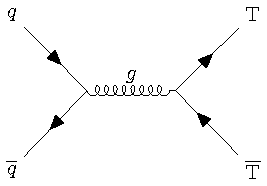
\includegraphics[width=0.6\linewidth]{Images/T_prod_qcd.pdf}
\captionof{figure}{Representative Feynman diagram for T pair production via gluon-mediated QCD processes.\label{fig:qcd_T_prod}}  
\end{center}

\begin{center}
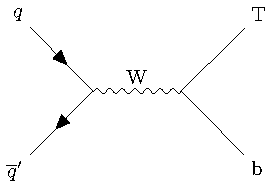
\includegraphics[width=0.6\linewidth]{Images/T_prod_qed.pdf}
\captionof{figure}{Representative Feynman diagram for single T production via electroweak processes.\label{fig:qed_T_prod}}  
\end{center}



In those studies, \textrm{T} decays into $\mathrm{bW}$, $\mathrm{tZ}$, or $\mathrm{tH}$ have been considered. In the context of \textrm{T} pair production, $\mathrm{T}\bar{\mathrm{T}}$, via QCD processes, the cross sections are well-known and solely depend on the mass of the vector-like quark.  Assuming a narrow $\mathrm{T}$ decay width ($\Gamma / m(\mathrm{T}) < 0.05$ or $0.1$) and a $100$\% branching fraction to $\textrm{bW}$, $\textrm{tZ}$, or $\textrm{tH}$, these searches have set stringent bounds on $m(\mathrm{T})$, excluding masses below almost $1.5$ \textrm{TeV} at $95$\% confidence level~\parencite{CMS:2024bni,CMS:2024qdd,ATLAS:2022ozf,ATLAS:2023bfh,ATLAS:2022hnn,ATLAS:2022tla,ATLAS:2023pja,ATLAS:2024fdw}. The most recent analysis from the CMS collaboration probes T-quark production via $\mathrm{pp} \to \mathrm{T}\textrm{qb}$, in final states with $\mathrm{T} \to \textrm{tZ}$ or $\mathrm{T} \to \textrm{tH}$, considering scenarios with preferential couplings to third-generation fermions. The analysis sets $95$\% confidence level upper limits of $68-1260$ \textrm{fb} on the production cross section, for T masses ranging from 600-1200 \textrm{GeV}~\parencite{CMS:2024qdd}. The latest studies from ATLAS probe vector-like quarks using the single-T production mode with the $\mathrm{T} \to \textrm{tH}$ decay channel leading to a fully hadronic final state~\parencite{ATLAS:2022ozf}, the single-\textrm{T} production mode with the $\mathrm{T} \to \textrm{tZ}$ decay channel leading to a multileptonic final state~\parencite{ATLAS:2023bfh}, the \textrm{TT} pair production mode with various \textrm{T} decay channels leading to multileptonic final states~\parencite{ATLAS:2022hnn}, and the \textrm{TT} pair production mode with various \textrm{T} decay channels leading to a single lepton plus missing momentum final state~\parencite{ATLAS:2022tla,ATLAS:2023pja}. 
The multilepton search offers the greatest sensitivity in most of the phase space, but the missing transverse energy based search has better sensitivity for low branching fraction $\mathfrak{B}(\mathrm{T}\to \textrm{Wb})$ and high $\mathfrak{B}(\mathrm{T}\to \textrm{Ht})$. These searches have similar sensitivities for the singlet and doublet models, resulting in exclusion bounds for masses below about $1.25$ \textrm{TeV} and $1.41$ \textrm{TeV}, respectively. 


A key consideration in the model interpretations summarized above is that the $\mathrm{T}$ branching fractions depend on the chosen model. The excluded mass range is less restrictive for specific branching fraction scenarios, such as $\{\mathfrak{B}(\mathrm{T} \to \textrm{tZ})$, $\mathfrak{B}(\mathrm{T} \to bW)$, $\mathfrak{B}(\mathrm{T} \to \textrm{tH})\}= \{0.2, 0.6, 0.2\}$, setting bounds on masses below about $0.95$ \textrm{TeV}. Moreover, if the $\mathrm{T} \to \phi't $ decay is allowed, or if the branching fractions $\mathfrak{B}(\mathrm{T} \to \textrm{tH/bW})$ are lower, the limits previously quoted must be re-evaluated. The authors of Ref.~\parencite{Cacciapaglia:2019zmj} emphasize that bounds on $m(\mathrm{T})$ can be around $500$ \textrm{GeV} when $\mathrm{T} \to \mathrm{t}\phi'$ decays are permitted. Therefore, to facilitate a comprehensive study, benchmark scenarios in this paper are considered down to $m(\chi_\mathrm{u}) = 500$ \textrm{GeV}.

\section{The Minimal $U(1)_{T_R^3}$ Model}\label{sec:model}

% \subsection{Scalar Potential}

The model extends the SM by an Abelian gauge symmetry $U(1)_{T^3_R}$, under which only the right-handed fermions are charged. The symmetry breaking is achieved via two independent Higgs mechanisms: one with the SM Higgs doublet $H$ for electroweak symmetry breaking, and another with a Higgs singlet $\phi$ for breaking $U(1)_{T^3_R}$. These scalars acquire independent vacuum expectation values (VEVs), $\langle H \rangle = v_h / \sqrt{2}$ and $\langle \phi \rangle = v_\phi / \sqrt{2}$. In the Kibble parametrization, the fields are written as:
\begin{align}
    H & = \begin{pmatrix}
        G_{+} \\
        \frac{1}{\sqrt{2}}\left(v_h + \rho_0 + i G_{0}\right)
    \end{pmatrix}, \label{eq:higgskibblepara1} \\
    \phi & = \frac{1}{\sqrt{2}}\left(v_\phi + \rho_\phi + i G_{\phi}\right). \label{eq:higgskibblepara2}
\end{align}
In Eqs.~\eqref{eq:higgskibblepara1} and~\eqref{eq:higgskibblepara2}, $G_\pm$, $G_0$, and $G_\phi$ are the Goldstone bosons absorbed by the SM $W^\pm$ and $Z$ bosons and the dark photon $A'$ (associated with $U(1)_{T^3_R}$) to acquire mass. The fields $\rho_h$ and $\rho_\phi$ mix to form the physical mass eigenstates, the SM-like Higgs boson $h$ and a dark Higgs $\phi'$:
\begin{equation}
    \begin{pmatrix}
        h \\
        \phi'
    \end{pmatrix}
    =
    \begin{pmatrix}
        \cos\alpha & -\sin\alpha \\
        \sin\alpha & \cos\alpha
    \end{pmatrix}
    \begin{pmatrix}
        \rho_0 \\
        \rho_\phi
    \end{pmatrix}.
\end{equation}
This mixing arises from diagonalizing the mass matrix derived from the gauge-invariant scalar potential:
\begin{equation}
    \begin{aligned}
        V(H, \phi) &= \mu_H^2 H^\dagger H + \mu_\phi^2 \phi^* \phi \\
                    &\quad + \lambda (H^\dagger H)(\phi^* \phi) + \lambda_H (H^\dagger H)^2 + \lambda_\phi (\phi^* \phi)^2.
    \end{aligned}
\end{equation}
Minimizing the potential yields the tadpole equations:
\begin{align}
    \frac{\partial V}{\partial H} &= \frac{v_h}{\sqrt{2}} \left( \mu_H^2 + \lambda_H v_h^2 + \frac{1}{2} \lambda v_\phi^2 \right) = 0, \\
    \frac{\partial V}{\partial \phi} &= \frac{v_\phi}{\sqrt{2}} \left( \mu_\phi^2 + \lambda_\phi v_\phi^2 + \frac{1}{2} \lambda v_h^2 \right) = 0.
\end{align}
The physical scalar masses are given by:
\begin{equation}
    m_{h,\phi'}^2 = \frac{1}{2} \left( \lambda_H v_h^2 + \lambda_\phi v_\phi^2 \right) \pm \sqrt{ \lambda^2 v_h^2 v_\phi^2 + \left( \lambda_H v_h^2 - \lambda_\phi v_\phi^2 \right)^2 },
\end{equation}
and the mixing angle $\alpha$ satisfies:
\begin{equation}
    \tan 2\alpha = \frac{-\lambda v_h v_\phi}{ \lambda_\phi v_\phi^2 - \lambda_H v_h^2}.
\end{equation}
The quartic couplings can be expressed in terms of the physical parameters:
\begin{align}
  \lambda_H &= \frac{m_{\phi'}^2 + m_h^2 + (m_{\phi'}^2 - m_h^2)\cos 2\alpha}{4 v_h^2}, \\
  \lambda_\phi &= \frac{m_{\phi'}^2 + m_h^2 + (m_{\phi'}^2 - m_h^2)\cos 2\alpha}{4 v_\phi^2}, \\
  \lambda &= \frac{m_{\phi'}^2 - m_h^2}{2 v_h v_\phi} \sin 2\alpha.
\end{align}
Thus, the scalar sector has four free parameters: the masses $m_h$ and $m_{\phi'}$, the mixing angle $\alpha$, and the dark Higgs VEV $v_\phi$. Similar to how $v_h$ is fixed by the electroweak gauge boson masses, $v_\phi$ is related to the dark photon mass by $m_{A'}^2 = g_{T^3_R}^2 v_\phi^2$, where $g_{T^3_R}$ is the $U(1)_{T^3_R}$ gauge coupling. Depending on the value of $g_{T^3_R}$, this gauge boson can behave as a heavy $Z'$ or a light dark photon. In this chapter, we assume $g_{T^3_R}$ is sufficiently small such that $A'$ can be treated as a dark photon.

\subsection{The Universal Seesaw Mechanism}

In this model, the masses of the SM fermions are generated through a universal seesaw mechanism by mixing with vector-like fermions $\chi_f$. The relevant mass terms in the Lagrangian are:
\begin{equation}
    -\mathcal{L} \supset Y_{f_L} \bar{f}_L' \chi_{fR}' H + Y_{f_R} \bar{\chi}_{fL}' f_R' \phi^* + m_{\chi_f'} \bar{\chi}_{f L}' \chi_{f R}' + \text{h.c.}
\end{equation}
This leads to the mass matrix:
\begin{equation}
    M_f = \begin{pmatrix}
        0 & Y_{f_L} v_h / \sqrt{2} \\
        Y_{f_R} v_\phi / \sqrt{2} & m_{\chi_f'}
    \end{pmatrix}.
\end{equation}
The mass eigenstates $(f, \chi_f)$ are obtained by rotating the gauge eigenstates:
\begin{equation}
    \begin{pmatrix}
        f_{L,R} \\
        \chi_{f_{L,R}}
    \end{pmatrix}
    =
    \begin{pmatrix}
        \pm \cos\theta_{f_{L,R}} & \mp \sin \theta_{f_{L,R}} \\
        \sin \theta_{f_{L,R}} & \cos\theta_{f_{L,R}}
    \end{pmatrix}
    \begin{pmatrix}
        f_{L,R}' \\
        \chi_{f_{L,R}}'
    \end{pmatrix},
\end{equation}
such that $\mathcal{R}(\theta_{f_L}) M_f \mathcal{R}^{-1}(\theta_{f_R}) = \text{diag}(m_f, m_{\chi_f})$. For real parameters, the physical masses and mixing angles are given by:
\begin{gather}
    m_f m_{\chi_f} = \frac{ Y_{f_L} v_h Y_{f_R} v_\phi }{2}, \label{eq:prodmass} \\
    m_f^2 + m_{\chi_f}^2 = m_{\chi_f'}^2 + \frac{1}{2} \left( Y_{f_L}^2 v_h^2 + Y_{f_R}^2 v_\phi^2 \right), \label{eq:summass} \\
    \tan \theta_{f_{L,R}} = \frac{\sqrt{2}}{m_{\chi_f'}} \left( \frac{Y_{f_{L,R}} v_{h,\phi}}{2} - \frac{m_f^2}{Y_{f_{L,R}} v_{h,\phi}} \right).
\end{gather}
The Yukawa interactions of the physical fermions with the scalars $h$ and $\phi'$ are:
\begin{equation}
    -\mathcal{L}_{\text{yuk}} = h \, \bar{\psi}_{f_L} \, \mathcal{Y}_{h} \, \psi_{f_R} + \phi' \, \bar{\psi}_{f_L} \, \mathcal{Y}_{\phi} \, \psi_{f_R},
\end{equation}
where $\psi_f = (f, \chi_f)^T$. The Yukawa matrices are:
\begin{align}
    \mathcal{Y}_{h} &= \frac{1}{\sqrt{2}} \mathcal{R}(\theta_{f_L}) \left( Y_{f_L} \sigma_+ \cos\alpha - Y_{f_R} \sigma_- \sin\alpha \right) \mathcal{R}^{-1}(\theta_{f_R}), \label{eq:YukawaL} \\
    \mathcal{Y}_{\phi} &= \frac{1}{\sqrt{2}} \mathcal{R}(\theta_{f_L}) \left( Y_{f_L} \sigma_+ \sin\alpha + Y_{f_R} \sigma_- \cos\alpha \right) \mathcal{R}^{-1}(\theta_{f_R}), \label{eq:YukawaR}
\end{align}
with $\sigma_{\pm} = (\sigma_1 \pm i \sigma_2)/2$ being the ladder Pauli matrices.

The expressions above provide a simplified, one-generation view. The complete model involves a non-trivial flavor structure where the mass matrices are general $3 \times 3$ matrices. The diagonalization of the full $6 \times 6$ mass matrices, the procedure for absorbing unphysical unitary rotations, and the emergence of the CKM matrix are detailed in Appendix~\ref{app:universal_seesaw}. Furthermore, the appendix contains a rigorous treatment of the mass eigenvalue problem, deriving the exact relationship between the fundamental parameters $(m_L, m_R, m_\chi)$ and the physical observables $(m_f, m_F, \theta_L)$, which leads to critical constraints on the model's parameter space to ensure perturbativity.



\subsection{Minimal UV-complete Theory}

To generate non-zero masses for all SM fermions and ensure gauge anomaly cancellation, the model must include at least one full generation of vector-like fermions $\{\chi_\mathrm{u}, \chi_\mathrm{d}, \chi_\mathrm{\ell}, \chi_\mathrm{\nu}\}$ and the right-handed neutrinos $\nu_R$ for each SM generation. Their quantum numbers are listed in Table~\ref{tab:QMnumbers}. The Yukawa interactions in the UV-complete theory are:
\begin{equation}
    \begin{aligned}
        -\mathcal{L} \supset&\,
        Y_{L u}^{ij} \bar{q}_L^{\prime i} \chi_{u R}^{\prime j} \widetilde{H}
        + Y_{R u}^{ij} \bar{\chi}_{u L}^{\prime i} u_R^{\prime j} \phi^*
        + m_{\chi_\mathrm{u}}^{ij} \bar{\chi}_{u L}^{\prime i} \chi_{u R}^{\prime j} \\
        &+ Y_{L d}^{ij} \bar{q}_L^{\prime i} \chi_{d R}^{\prime j} H
        + Y_{R d}^{ij} \bar{\chi}_{d L}^{\prime i} d_R^{\prime j} \phi
        + m_{\chi_d}^{ij} \bar{\chi}_{d L}^{\prime i} \chi_{d R}^{\prime j} \\
        &+ Y_{L \ell}^{ij} \bar{\ell}_L^{\prime i} \chi_{\ell R}^{\prime j} H
        + Y_{R \ell}^{ij} \bar{\chi}_{\ell L}^{\prime i} \ell_R^{\prime j} \phi
        + m_{\chi_\ell}^{ij} \bar{\chi}_{\ell L}^{\prime i} \chi_{\ell R}^{\prime j} \\
        &+ Y_{L \nu}^{ij} \bar{\ell}_L^{\prime i} \chi_{\nu R}^{\prime j} \widetilde{H}
        + Y_{R \nu}^{ij} \bar{\chi}_{\nu L}^{\prime i} \nu_R^{\prime j} \phi^*
        + m_{\chi_\nu}^{ij} \bar{\chi}_{\nu L}^{\prime i} \chi_{\nu R}^{\prime j}
        + \text{h.c.}
    \end{aligned}
\end{equation}
Here, $i, j = 1,2,3$ are generation indices. The diagonalization of the mass matrices for each fermion type follows the structure outlined in Eqs.~\eqref{eq:prodmass} and~\eqref{eq:summass}, while the Yukawa matrices generalize the structure of Eqs.~\eqref{eq:YukawaL} and~\eqref{eq:YukawaR}, now encoding the CKM and PMNS mixing matrices. The neutrino sector has a more complex structure due to the possibility of a Majorana mass term for the vector-like neutrinos $\chi_\nu'$.

\begin{table}[h!]
    \centering
    \begin{tabular}{ccccc}
        \hline
        \hline
        Field & $SU(3)_C$  & $SU(2)_L$ & $U(1)_Y$ & $U(1)_{T^3_R}$ \\
        \hline\hline
        $q_L'$                    & \textbf{3} & \textbf{2} & 1/6 & 0\\
        $\ell_L'$                 & \textbf{1} & \textbf{2} & -1/2 & 0\\
        $H$                       & \textbf{1} & \textbf{2} & 1/2 & 0\\
        \hline
        $u_R^{\prime c}$          & \textbf{3} & \textbf{1} & -2/3 & -2\\
        $d_R^{\prime c}$          & \textbf{3} & \textbf{1} & 1/3 & 2\\
        $\ell_R^{\prime c}$       & \textbf{1} & \textbf{1} & 1 & 2\\
        $\nu_R^{\prime c}$        & \textbf{1} & \textbf{1} & 0 & -2\\
        $\phi$                    & \textbf{1} & \textbf{1} & 0 & 2\\
        \hline
        $\chi_{u_L}'$             & \textbf{3} & \textbf{1} & 2/3 & 0\\
        $\chi_{u_R}^{\prime c}$   & \textbf{3} & \textbf{1} & -2/3 & 0\\
        $\chi_{d_L}'$             & \textbf{3} & \textbf{1} & -1/3 & 0\\
        $\chi_{d_R}^{\prime c}$   & \textbf{3} & \textbf{1} & 1/3 & 0\\
        $\chi_{\ell_L}'$          & \textbf{1} & \textbf{1} & -1 & 0\\
        $\chi_{\ell_R}^{\prime c}$& \textbf{1} & \textbf{1} & 1 & 0\\
        $\chi_{\nu_L}'$           & \textbf{1} & \textbf{1} & 0 & 0\\
        $\chi_{\nu_R}^{\prime c}$ & \textbf{1} & \textbf{1} & 0 & 0\\
        \hline
        \hline
    \end{tabular}
    \caption{Minimal field content of the model and their representations under the SM and $U(1)_{T^3_R}$ gauge groups.}
    \label{tab:QMnumbers}
\end{table}


\section{Samples and Simulation}\label{sec:sims}


The minimal $U(1)_{T^3_R}$ model described in Sec.~\ref{sec:model} is implemented \textit{at tree level} into the \texttt{FeynRules} package~\parencite{Alloul:2013bka}, which generates the Feynman rules and exports them into a Universal \texttt{FeynRules} Output (\texttt{UFO})~\parencite{Degrande:2011ua}. The resulting \texttt{UFO} is utilized as input for a generator to produce the MC samples. Both signal and background events are generated with the \texttt{MadGraph5\_aMC@NLO} v3.2.0 program~\parencite{Alwall:2014hca,Alwall:2014bza} at leading order (LO) in QCD, considering \textrm{pp} beams colliding with a center-of-mass energy of $\sqrt{s} = 13.6$ \textrm{TeV}. Each signal and background sample is generated separately, with no interference effects between the signal and background considered. The impact of these interference effects has been evaluated, and for all values of $\chi_\mathrm{u}$ and $\phi'$ masses considered, the effect on the signal plus background cross section is found to be less than $<0.5$\%. Additionally, the effect on the shape of the b-jet $p_{T}$ distribution is less than 6\% for $p_{T} < 300$ GeV and less than 2\% for b-jet $p_{T} > 300$ GeV. We use the \texttt{NNPDF3.0~NLO}~\parencite{NNPDF:2014otw} set for parton distribution functions (PDFs) for all event generation. Parton-level events are then interfaced with \texttt{PYTHIA} (v8.2.44)~\parencite{Sjostrand:2014zea} to account for parton showering and hadronization processes. Finally, we use  \texttt{DELPHES} (v3.4.2)~\parencite{deFavereau:2013fsa} to simulate smearing and other detector effects using the CMS detector geometric configurations and parameters for particle identification and reconstruction, using the CMS input card with 140 average pileup interactions.

\begin{center}
  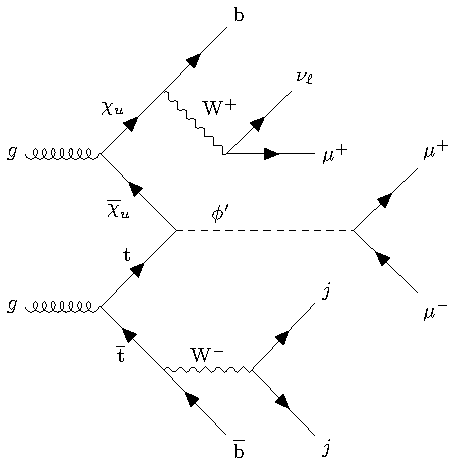
\includegraphics[width=0.75\linewidth]{Images/signal_qqfusion.pdf}
    \captionof{figure}{Representative Feynman diagram for the production of a $\phi'$ boson in association with a $\chi_\mathrm{u}$ vector-like quark through the fusion of a top quark and $\chi_\mathrm{u}$ vector-like quark. Once again, the $\phi'$ decays to a pair of muons, the top quark decays fully hadronically, and the $\chi_\mathrm{u}$ decays semi-leptonically to muons, neutrinos and $b$-jets.\label{fig:qqfusion}}
\end{center}

\begin{center}
    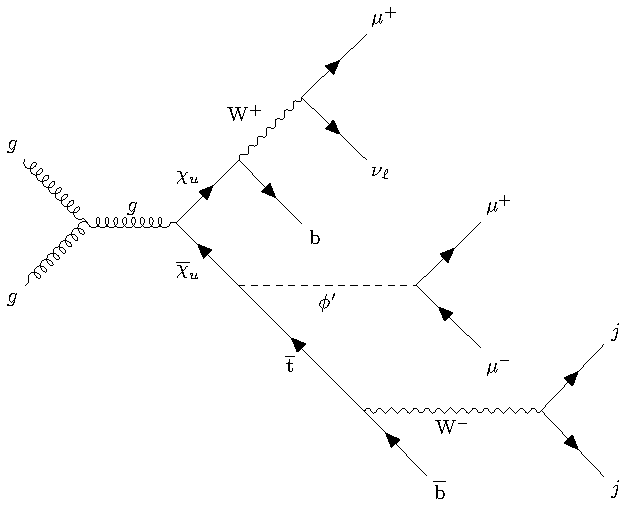
\includegraphics[width=0.85\linewidth]{Images/signal_ggfusion.pdf}
    \captionof{figure}{Representative Feynman diagram for the production of a $\phi'$ boson in association with a $\chi_\mathrm{u}$ vector-like quark through the fusion of a gluon pair from incoming protons. The $\phi'$ decays to a pair of muons, the top quark that decays fully hadronically, and the $\chi_\mathrm{u}$ decay semi-leptonically to muons, neutrinos and jets.\label{fig:ggfusion}}
\end{center}

All signal cross sections used in this analysis are obtained requiring the following kinematic criteria on leptons $\ell$, \textrm{b} quarks, and light-quark/gluon jets ($j$) at parton level in \texttt{MadGraph}: $p_{\mathrm{T}}(\ell) > 35$~\textrm{GeV}, $\abs{\eta (\mathrm{b})} < 2.5$, $\abs{\eta (\ell)} < 2.3$, $p_{\mathrm{T}}(j) > 20$~\textrm{GeV}, and $\abs{\eta (\mathrm{j})} < 5$. These parton-level selections were applied exclusively to the signal processes to restrict event generation to the relevant phase space regions. For background processes, these default parton level requirements in \texttt{MadGraph} were imposed:  $p_{\mathrm{T}}(\ell) > 10$~\textrm{GeV}, $\abs{\eta (\ell)} < 2.5$, $p_{\mathrm{T}}(j) > 20$~\textrm{GeV}, $\abs{\eta (\mathrm{j})} < 5$, and $\abs{\eta (\mathrm{b})} < 5$. This ensures that the phase space regions for the background near the analysis-level selection criteria are adequately described after parton showering since the pre-selections at the analysis level are more stringent than the parton-level requirements. Furthermore, we use the MLM algorithm for jet matching and jet merging. The parameters \texttt{xqcut} and \texttt{qcut} of the MLM algorithm are set to 30 and 45 respectively to ensure continuity of the differential jet rate as a function of jet multiplicity. Each simulated signal and background sample is produced separately at LO, with one million events at the generation level, neglecting potential interference effects between the signal and background due to the suppression caused by the different orders of magnitude in the coupling constants of the signal and background.

Signal samples are generated considering the production of a $\phi'$ boson, an associated $\chi_\mathrm{u}$ vector-like quark, and a top quark $(\mathrm{pp}\to \chi_\mathrm{u} \mathrm{t} \phi')$, inclusive in both $\alpha$ and $\alpha_s$ (see Figures~\ref{fig:qqfusion}-\ref{fig:ggfusion}). We have used the implementation of the $U(1)_{T^3_R}$ model in Ref.~\parencite{Dutta2023}. Signal samples were created considering coupling values of $Y_{\mathrm{t}_R}=Y_{\mathrm{t}_L}=2\sqrt{2}$ in the range of masses $m(\phi')\in\{5,10,50,100,325\}$~\textrm{GeV} for the dark higgs and $m(\chi_\mathrm{u})\in\{0.50, 0.75, 1.0, 1.5, 2.0, $ $ 2.5\}$~\textrm{TeV} for the vector-like quark $\chi_u$~\parencite{PhysRevD.108.095006}. The production cross section for $\mathrm{pp}\to \chi_\mathrm{u} \mathrm{t} \phi'$ is highly dependent on the choice of the Yukawa couplings in the Lagrangian. The ${\chi_\mathrm{u}}{- \mathrm{t}}$ fusion process shown in Fig.~\ref{fig:qqfusion} is dominated by the $Y_{\mathrm{t}_R}$ coupling. However, the decay ${\chi_\mathrm{u}} \to \mathrm{t} \phi'$ shown in Fig.~\ref{fig:ggfusion} is inversely proportional to the $Y_{\mathrm{t}_L}$ coupling. This effect is shown in Fig.~\ref{fig:cross_section_by_lambdas}, which displays the total signal cross section, as a function of $Y_{\mathrm{t}_R}$ and $Y_{\mathrm{t}_L}$, for a benchmark point with $m(\phi')=100$~\textrm{GeV} and $m(\chi_\mathrm{u})=1.0$~\textrm{TeV}. 

\begin{figure}
    \centering
    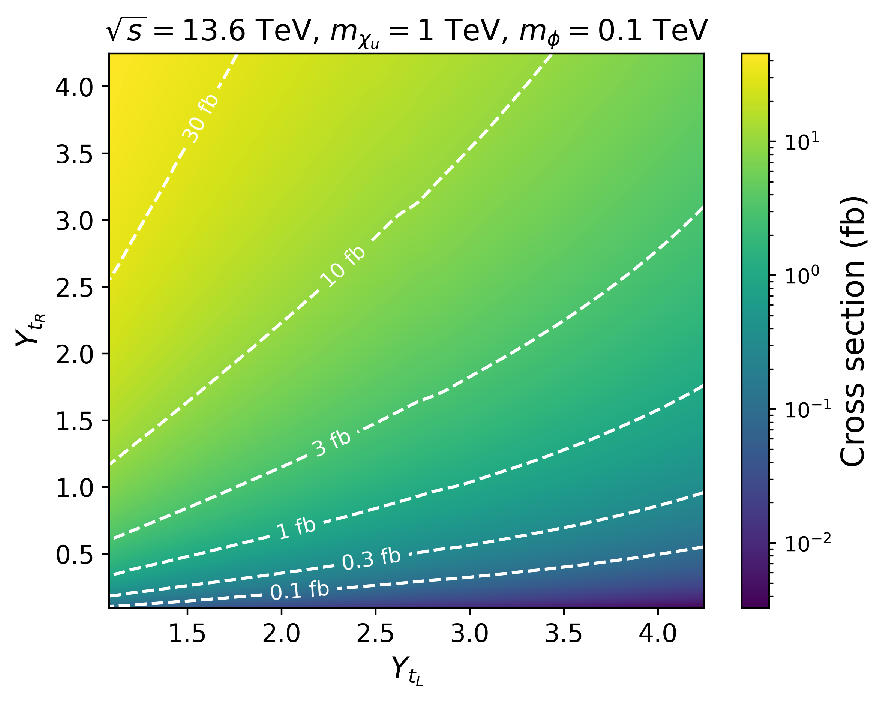
\includegraphics[width=0.85\linewidth]{Images/cross_section_by_lambdas.pdf}
    \caption{Signal production cross section, $ \mathrm{pp}\to \chi_\mathrm{u} \mathrm{t} \phi'$,  in the $Y_{\mathrm{t}_R}$ versus $Y_{\mathrm{t}_L}$ plane, for a benchmark point with $m(\phi')=100$~\textrm{GeV} and $m(\chi_\mathrm{u})=1.00$~\textrm{TeV}. The white-dashed contours show specific cross section values in the two dimensional plane.}
    \label{fig:cross_section_by_lambdas}
\end{figure}

We target signal events where the top quark decays hadronically into a bottom quark and two jets ($\mathrm{t} \to \mathrm{bW} \to \mathrm{b} q \bar{q}'$), the $\chi_\mathrm{u}$ decays semileptonically into a $b$ quark, lepton, and neutrino (via $\chi_\mathrm{u} \to \mathrm{bW}$ and $\mathrm{W}\to\mu\nu_{\mu}$), and the $\phi'$ produces two muons. We note that the scalar $\phi'$ particle could result from the mixture of the SM Higgs boson and additional scalar fields, and the Yukawas of the fermions could additionally arise from the mixing of the SM fermions with additional copies of the associated vector-like fermions. Therefore, the $\phi'$ branching ratios are dependent on the chosen mechanism and model by which this mixture occurs, see for example, Refs.~\parencite{Cacciapaglia_2023,Blankenburg:2012nx,Jones-Perez:2013oia,Calibbi:2009pv}. For the purpose of this work, and 
similar to Refs.~\parencite{Dutta2020,Dutta2023}, the considered benchmark signal scenarios have $\mathfrak{B}(\chi_\mathrm{u} \rightarrow \textrm{b W})$ of about 0.5 and $\mathfrak{B}(\phi' \rightarrow \mu^+\mu^-)=1.00$. Fig.~\ref{fig:xs-plot} shows the production cross section in \textrm{fb}, as a function of $m(\phi')$ and $m(\chi_\mathrm{u})$ masses, assuming the aforementioned decays, branching ratios, and couplings.

We note that for the parameter space of focus in this paper, the total mass of the $t$-$\chi_\mathrm{u}$ system is larger than $m(\phi')$, thus the large rest energy of the $t$-$\chi_\mathrm{u}$ system is converted into potentially large momentum values for the $\phi'$. Similarly, the $t$-quark produced through the $\chi_\mathrm{u}$-$t$ fusion interaction can also have large momentum values, and thus in some cases the hadronic $t$ decay products cannot be fully reconstructed independently of each other. This results in three possible $t$ reconstruction scenarios: a fully merged scenario where the $\mathrm{W}\to jj$ system and the $\mathrm{b}$ quarks are very collimated and reconstructed as a single ``fat jet’’ (henceforth referred to as a FatJet, FJ); a partially merged scenario, where the decay products of the $\mathrm{W}$ boson form a single FatJet but the $\mathrm{b}$ quark can still be separately identified; and an un-merged scenario where all decay products can be independently identified. Jets are clustered using the anti-$k_t$ algorithm~\parencite{Cacciari_2008} using the \texttt{FastJet} (v3.4.2)~\parencite{Cacciari_2012} package with a distance parameter of $R = 0.4$ for standard jets and $R = 0.8$ for fat jet objects. Each scenario has an associated identification efficiency and misidentification rate, which depends on the choice of the boosted $t$/$W$ algorithm (our choice of efficiency and misidentification rates is described later). 

Based on the above details, the final state of interest in this paper consists of three muons (two from the $\phi'$ decay and one from the $\chi_\mathrm{u}$ decay), a (possibly boosted) top-tagged system, at least one $b$-tagged jet, and large missing transverse momentum ($\vec{p}_{T}^{\textrm{~miss}}$). For the partially merged and un-merged scenarios, there will be two $b$ quarks present in the final state (one of which is part of the top tagged system). 

We consider background sources from SM processes which can give similar objects in the final state as those expected for signal. Several background sources were considered and studied, such as QCD multijet events, production of vector boson pairs ($\mathrm{VV: WW, ZZ, WZ}$), vector boson triplets ($\mathrm{VVV: WWZ, WZZ, ZZZ, WWW}$), top-quark pairs in association with weak bosons ($\mathrm{t}\overline{\mathrm{t}}X$), and $\mathrm{t}\overline{\mathrm{t}}\mathrm{t}\overline{\mathrm{t}}$ processes. The  dominant sources of SM background events are from the $\mathrm{t}\overline{\mathrm{t}}X$, $\mathrm{ZZW}$, and $\mathrm{t}\overline{\mathrm{t}}\mathrm{t}\overline{\mathrm{t}}$ processes. The $\mathrm{t}\overline{\mathrm{t}}X$ background is primarily associated production of a $\mathrm{Z}/\gamma^{*}$ from $\mathrm{t}\bar{\mathrm{t}}$ fusion processes. The $\mathrm{ZZW}$ process becomes a background when one $\mathrm{Z}$ decays $\mathrm{b}\bar{\mathrm{b}}$, another $\mathrm{Z}$ decays to a pair of muons, and the W decays to a muon and a neutrino. 
Events from $\mathrm{ZZW}$ and $\mathrm{t}\overline{\mathrm{t}}\mathrm{t}\overline{\mathrm{t}}$ have been combined, after being weighted by their corresponding production cross section. The combination is presented as the ``$\mathrm{b} \overline{\mathrm{b}}\mu\mu\mu\nu$'' background in the remainder of this paper. The $\mathrm{t}\overline{\mathrm{t}}X$ process is presented as part of the ``$\mathrm{t}\overline{\mathrm{t}}\mu^{+}\mu^{-}$'' background. Tab.~\ref{tab:dominantbkgs} shows the production cross sections for the dominant background sources. The rest of the aforementioned background processes do not contribute meaningfully in our context, accounting for $\ll 1\%$ of the total expected background yield.

The identification of leptons, boosted top quarks, and bottom quarks plays an important role in the ability to identify signal events, the ability to minimize the rate of SM backgrounds, and thus also the discovery reach in the high-luminosity environment of the LHC. It is worth noting that the reconstruction and identification of leptons and the decay products of the top/bottom quarks may be non-trivial at the High-Luminosity LHC (HL-LHC) due to the presence of a potentially large number of secondary pp interactions (pileup). The impact of pileup on the new physics discovery reach, and the importance of pileup mitigation at CMS and ATLAS has been outlined in many papers, for example in Ref.~\parencite{CMS-PAS-FTR-13-014}. We note the expected performance of the upgraded ATLAS and CMS detectors for the HL-LHC is beyond the scope of this work; however, the studies presented here do attempt to provide reasonable expectations by conservatively assuming some degradation in lepton and hadron identification efficiencies, using Ref.~\parencite{CMS-PAS-FTR-13-014} as a benchmark, and considering the case of 140 average pileup interactions. 

For muons with $|\eta|< 1.5$, the assumed identification efficiency is 95\% with a 0.3\% misidentification rate~\parencite{CMS-PAS-FTR-13-014,CMS_MUON_17001}. The performance degrades linearly with $\eta$ for $1.5 < |\eta| < 2.5$, and we assume an identification efficiency of 65\% with a 0.5\% misidentification rate at $|\eta| = 2.5$. Similarly, the charged hadron tracking efficiency, which contributes to the jet clustering algorithm and missing transverse momentum ($\vec{p}_{T}^{\textrm{~miss}}$) calculation, is 97\% for $1.5 < |\eta| < 2.5$, and degrades to about 85\% at $|\eta| = 2.5$. These potential inefficiencies due to the presence of secondary pp interactions contribute to how well the lepton and top kinematics can be reconstructed. Following Refs.~\parencite{CMS:2020poo,ATLAS:2018wis}, we consider the ``Loose'' working point for the identification of the fully merged (partially merged) $\mathrm{t}$ decays, which results in 80-85\% top (W) identification efficiency and 11-25\% misidentification rate, depending on the FatJet transverse momentum ($p_{T}^{FJ}$). Following Ref.~\parencite{CMSbtag}, we consider the ``Loose'' working point of the DeepCSV algorithm~\parencite{Bols_2020}, which gives a 70-80\% b-tagging efficiency and 10\% light quark mis-identification rate. The choice of boosted $t$/$W$ and b-tagging working points is determined through an optimization process that maximizes discovery reach. It is noted the contribution from SM backgrounds with a misidentified boosted $t$/$W$ is negligible, and thus our discovery projections are not sensitive to uncertainties related to the boosted $t$/$W$ misidentification rates. 

\begin{figure}
    \centering
    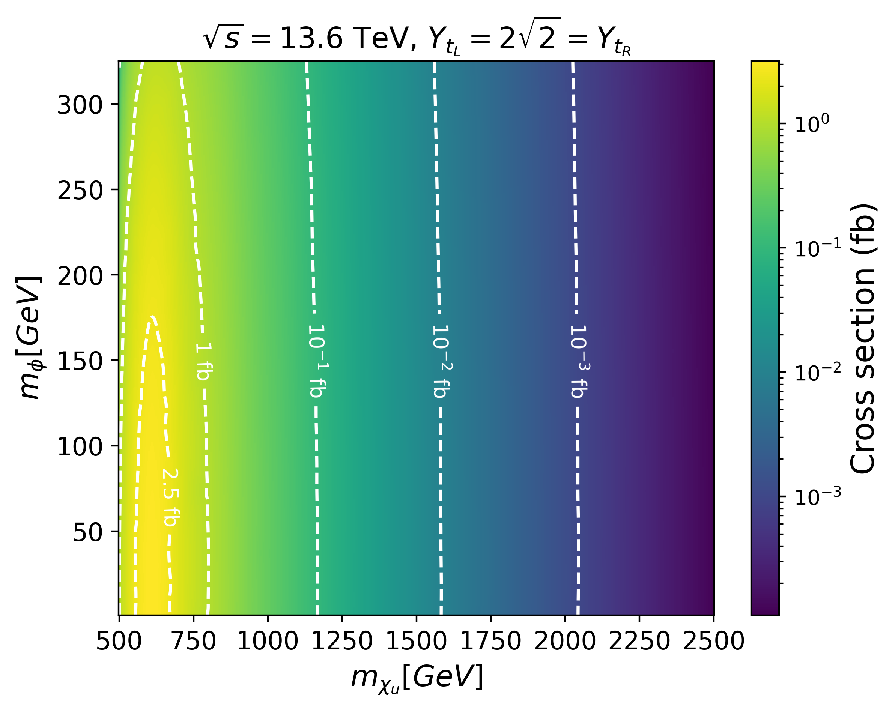
\includegraphics[width=0.85\linewidth]{Images/cross_section_by_masses.pdf}
    \caption{Projected cross section (fb) plot for $pp\to t \chi_\mathrm{u} \phi'$ and subsequent decay as a function of $m(\chi_\mathrm{u})$ and $m(\phi')$.}
    \label{fig:xs-plot}
\end{figure}

\begin{table}[]
  \begin{tabular}{l r}
    \hline
    {Background Process} & {Cross-Section $\sigma$ [\textrm{pb}]} \\
    \hline
   $\mathrm{pp} \to \mathrm{t} \overline{\mathrm{t}} \, \mu^+ \mu^-$ & $2.574\times 10^{-3}$  \\
    $\mathrm{pp} \to \mathrm{b}\overline{\mathrm{b}}\, \mu\mu\mu\nu $ & $4.692 \times 10^{-4}$ \\
    \hline
  \end{tabular}
  \centering
  \caption{A summary of dominant SM backgrounds produced by $\mathrm{pp}$ collisions and their cross sections in pb, as computed by \texttt{MadGraph} with $n = 10^6$ events.}
  \label{tab:dominantbkgs}
\end{table}

\begin{figure}[]
\centering
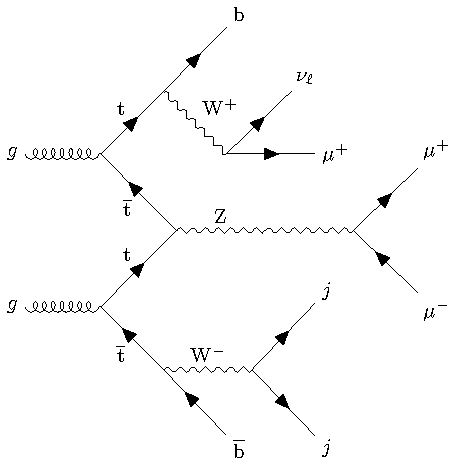
\includegraphics[width=.75\linewidth]{Images/bg_Z_full.pdf}
\caption{Representative Feynman diagram for a background event. A $Z$ boson is produced in association with a top quark through the fusion of a top, anti top pair from incoming protons. The $Z$ boson subsequently decays to a pair of muons and the two spectator top quarks decay semi-leptonically and purely hadronically to muons, neutrinos and jets, resulting in the same final states as the signal event.\label{fig:v}}
\end{figure}


\section{Data Analysis Using Machine Learning}\label{sec:ML}
The analysis of signal and background events is performed utilizing machine learning techniques. A machine learning-based approach offers sizeable advantages when compared to traditional event classification techniques. Unlike conventional methods, machine learning models have the capability to simultaneously consider all kinematic variables, allowing them to efficiently navigate the complex and high-dimensional space of event kinematics. Consequently, machine learning models can effectively enact sophisticated selection criteria that take into account the entirety of this high-dimensional space. This makes them ideal for high-energy physics applications.

The BDT method is a powerful machine learning technique that has proven its effectiveness in various applications, particularly in the field of collider physics. In this method, decision trees are trained greedily in a sequential manner, with each tree focusing on learning the discrepancies or residuals between its predictions and the expected values obtained from the previously trained tree. This iterative process aims to progressively minimize errors, making BDTs a particularly effective approach for enhancing model performance.

In the context of collider physics, BDTs have demonstrated their utility in addressing classification problems. In particular, BDTs can effectively discriminate between signal and background events, enabling accurate and efficient event classification. Their ability to handle subtle non-linear relationships within the data with high interpretability makes BDTs a valuable tool to handle large amounts of data with a large number of parameters for each event. 

The first step in our workflow involves the use of a specialized \texttt{MadAnalysis Expert Mode} C++ script~\parencite{CONTE2013222}. This script extracts essential kinematic and topological information from the simulated samples. The script will process the aforementioned variables contained within these files and transform them into a structured and informative CSV (Comma-Separated Values) format that can be used to train our machine learning models. These kinematic variables include crucial details about the events, such as particle momenta, energies, and topologies, providing the fundamental building blocks for our machine learning analysis. 

To account for the differential significance of various events, we apply cross-section weighting. This ensures that the relative importance of signal and background events is appropriately balanced in the dataset. This weighting is crucial for addressing the varying likelihood of observing different types of events in high-energy physics experiments. The prepared and weighted datasets are then passed to our \texttt{MadAnalysis Expert Mode} C++ script, where the simulated signal and background events are initially filtered, before being passed to the CSV file for use by the machine learning algorithm. The filtering process requires at least one well-reconstructed and identified $\mathrm{b}$-jet candidate, at least one jet (regular or FJ) not tagged as a $\mathrm{b}$ jet, and exactly three identified muons. The filtering selections are motivated by experimental constraints, such as the geometric constraints of the CMS/ATLAS detectors, the typical kinematic thresholds for the reconstruction of particle objects, and the available lepton triggers which also drive the minimal kinematic thresholds. Selected jets must have $p_{\mathrm{T}} > 30$ $\textrm{GeV}$ and $|\eta(j)| < 5.0$, while $\mathrm{b}$-jet candidates with $p_{\mathrm{T}} > 20$ $\textrm{GeV}$ and $|\eta(\mathrm{b})| < 2.5$ are chosen. The $\mu$ object must pass a $p_{\mathrm{T}} > 35$ $\textrm{GeV}$ threshold and be within a $|\eta(\ell)| < 2.3$. We will refer to this filtering criteria as pre-selections. The efficiency of the pre-selections depends on $m(\phi')$ and $m(\chi_{\mathrm{u}})$, but is typically about $25-30$\% for the signal samples. Events passing this pre-selection are used as input for the machine learning algorithm, which classifies them as signal or background, using a probability factor. 



We explore the performance of a diverse set of machine learning models, specifically three neural networks of differing architectures and a BDT algorithm. To ensure robust model assessment, we employed a standard 90-10 train-test split of the dataset, partitioning it into a 90\% portion for training and a 10\% portion for testing. This division allows us to gauge the generalization capabilities of our models on unseen data.  

The training and evaluation of the BDT were carried out in a high-performance computing environment. Specifically, an Nvidia A100 GPU was used. The canonical \texttt{PyTorch}~\parencite{paszke2019} deep learning framework was employed for configuring, training, and evaluating the neural networks. PyTorch is well-regarded for its flexibility and performance in deep learning applications.

For the BDT algorithm, we used hyperparameters $\eta=0.3$, $\gamma = 0$, and $\texttt{max\_depth} = 6$. The \texttt{XGBoost}~\parencite{chen_xgboost_2016} library was used for the implementation of the Boosted Decision Tree algorithm. It offers high efficiency, optimization, and interpretability, making it a suitable choice for this particular task. 



\begin{table}
    \centering
    \begin{tabular}{c  c  c}
    \hline
    { Model} & { Train/Test Acc. } & { Training Time} \\
    \hline
    \small
    BDT & N.A./0.9993  & 6s\\
    Neural Network 1 & 0.9999/0.9997 & 1h 58m \\
    Neural Network 2 & 0.9999/0.9998 & 2h 12m \\
    Neural Network 3 & 0.9999/0.9998 & 2h 32m\\
    \hline
    \end{tabular}
    \caption{Train/test results for the ML models.}\label{tab:ml_results}
    \centering
\end{table}

It is worth mentioning that we experimented with deep neural networks of various architectures. Although we found that they yield similar signal sensitivity to the BDT, the complex nature of the studies in this
work (particle objects considered, experimental constraints in a high luminosity LHC, etc.) motivates the use of a BDT over a deep neural network because of its usefulness, efficiency, and simplicity in understanding the machine learning output in addition to significantly shorter training times. Therefore, we perform our proceeding analysis using the BDT. The outcomes of our model training and evaluation are presented in Table 3. 

\section{Results}\label{sec:results}
Figures~\ref{fig:_mu12},~\ref{fig:pTb1}, and~\ref{fig:pTmu1} show relevant kinematic distributions for two benchmark signal points and the dominant SM backgrounds, using the subset of events passing the pre-selections defined above. The signal benchmark points in these figures are $m(\phi^{'}) = 325 \, \mathrm{GeV}$, $m(\chi_{\mathrm{u}}) = 2\, \mathrm{TeV}$, and $m(\phi^{'}) = 1 \, \mathrm{GeV}$, $m(\chi_{\mathrm{u}}) = 500\, \mathrm{GeV}$. The distributions are normalized such that the area under the curve is unity. These distributions correspond to the reconstructed mass, $m(\mu_{1}, \mu_{2})$, between the two muon candidates with the highest transverse momentum ($\mu_{1}$ and $\mu_{2}$), 
the transverse momentum of the \textrm{b}-jet candidate with the highest transverse momentum $p_{\mathrm{T}}$ ($\mathrm{b_{1}}$), and the muon candidate with the highest transverse momentum $p_{\mathrm{T}}$ ($\mu_{1}$), respectively. 
Note that the signal distributions exhibit tails that are significantly the backgrounds. These distributions are among the variables identified by the BDT algorithm with the highest signal to background discrimination power.


\begin{figure}
\centering
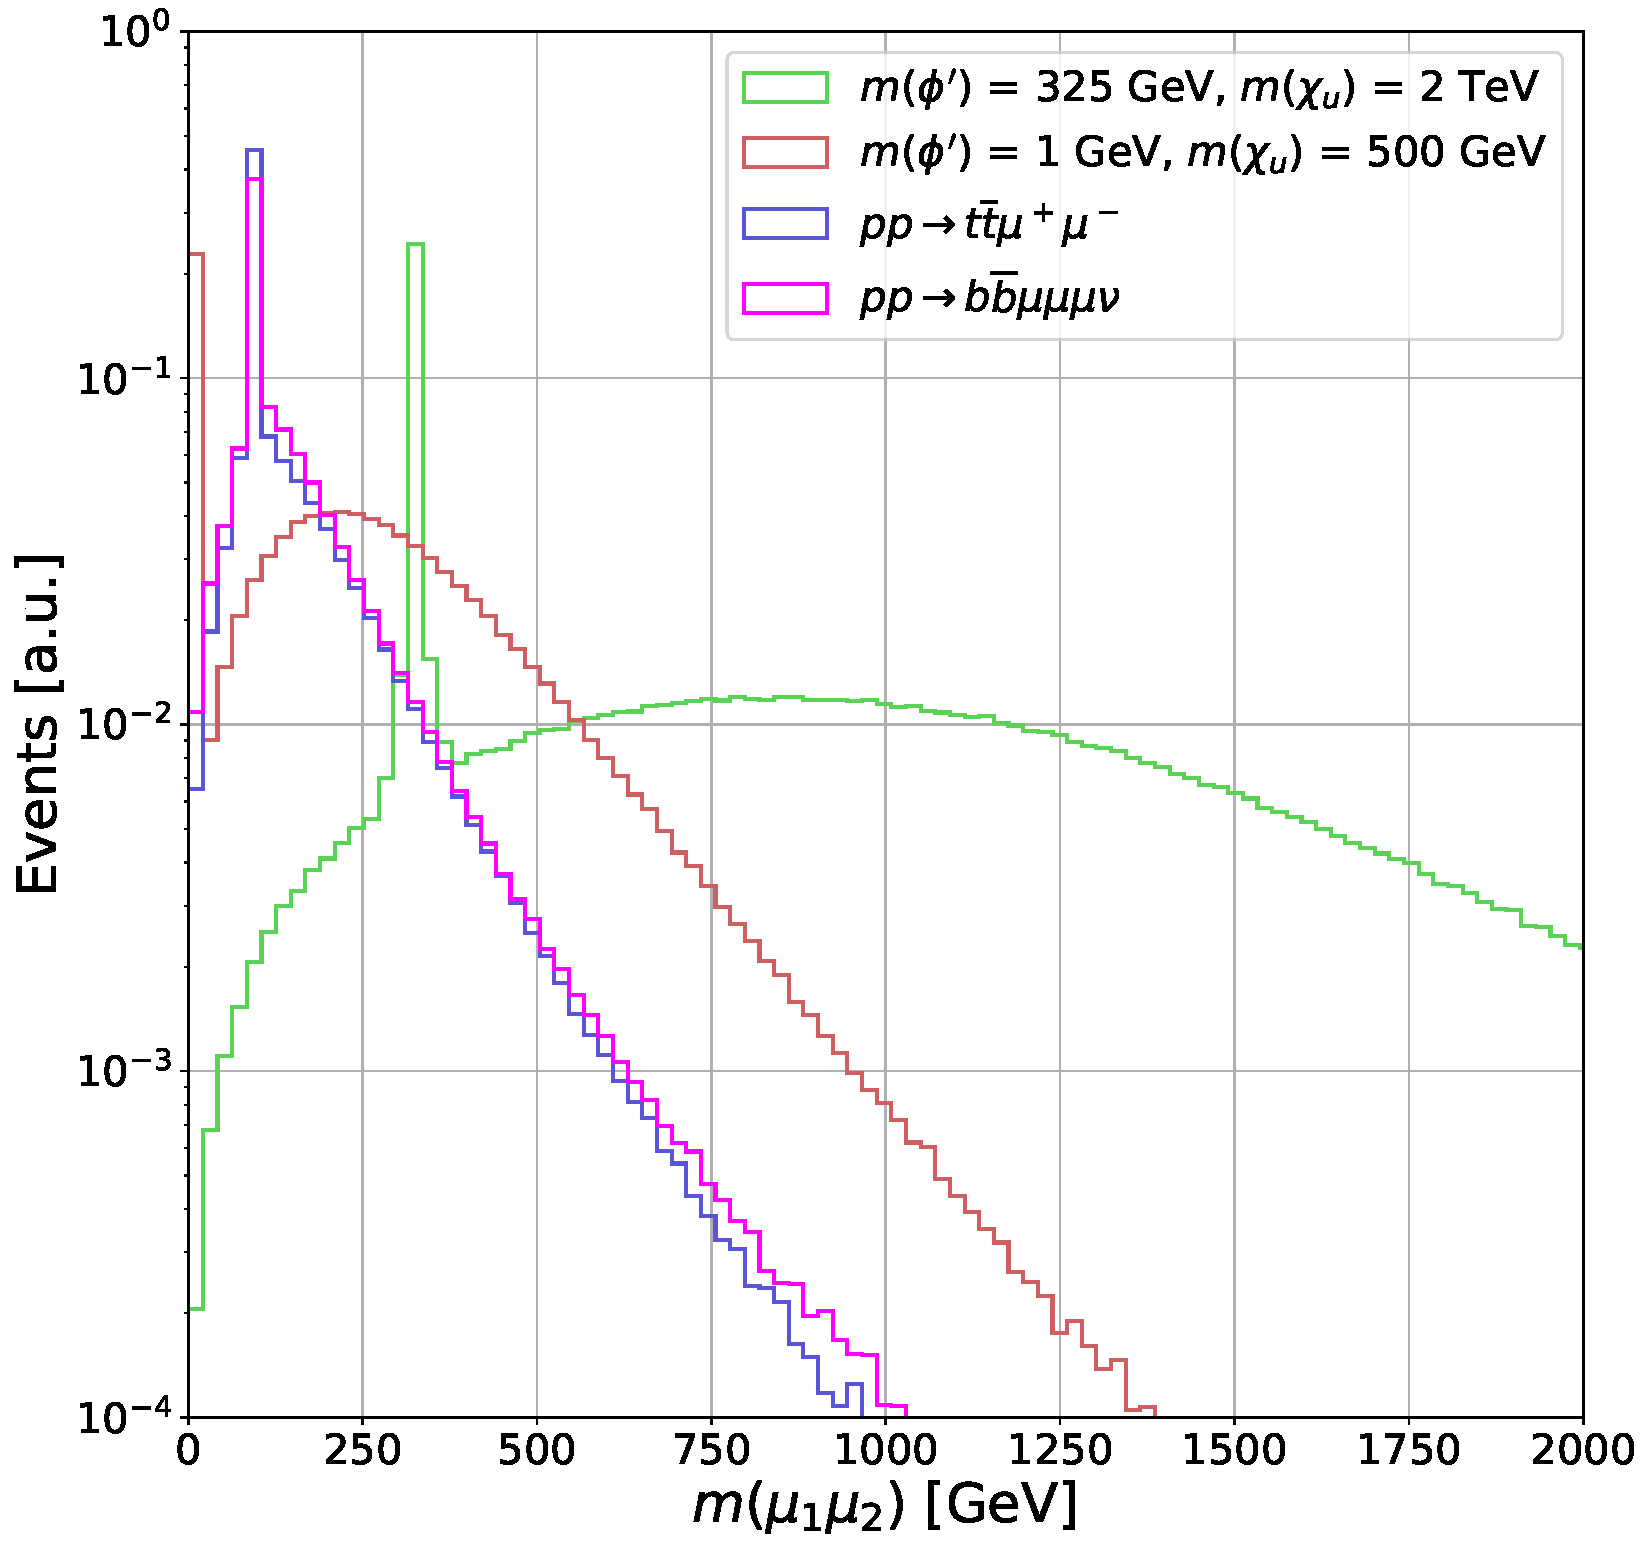
\includegraphics[width=.75\linewidth]{Images/M_mu_1_2.pdf}
\caption{Invariant mass distribution of the muon pair with the highest and second highest transverse momentum. The distributions are shown for the two main SM background processes and two signal benchmark points.\label{fig:_mu12}}
\end{figure}

\begin{figure}
\centering
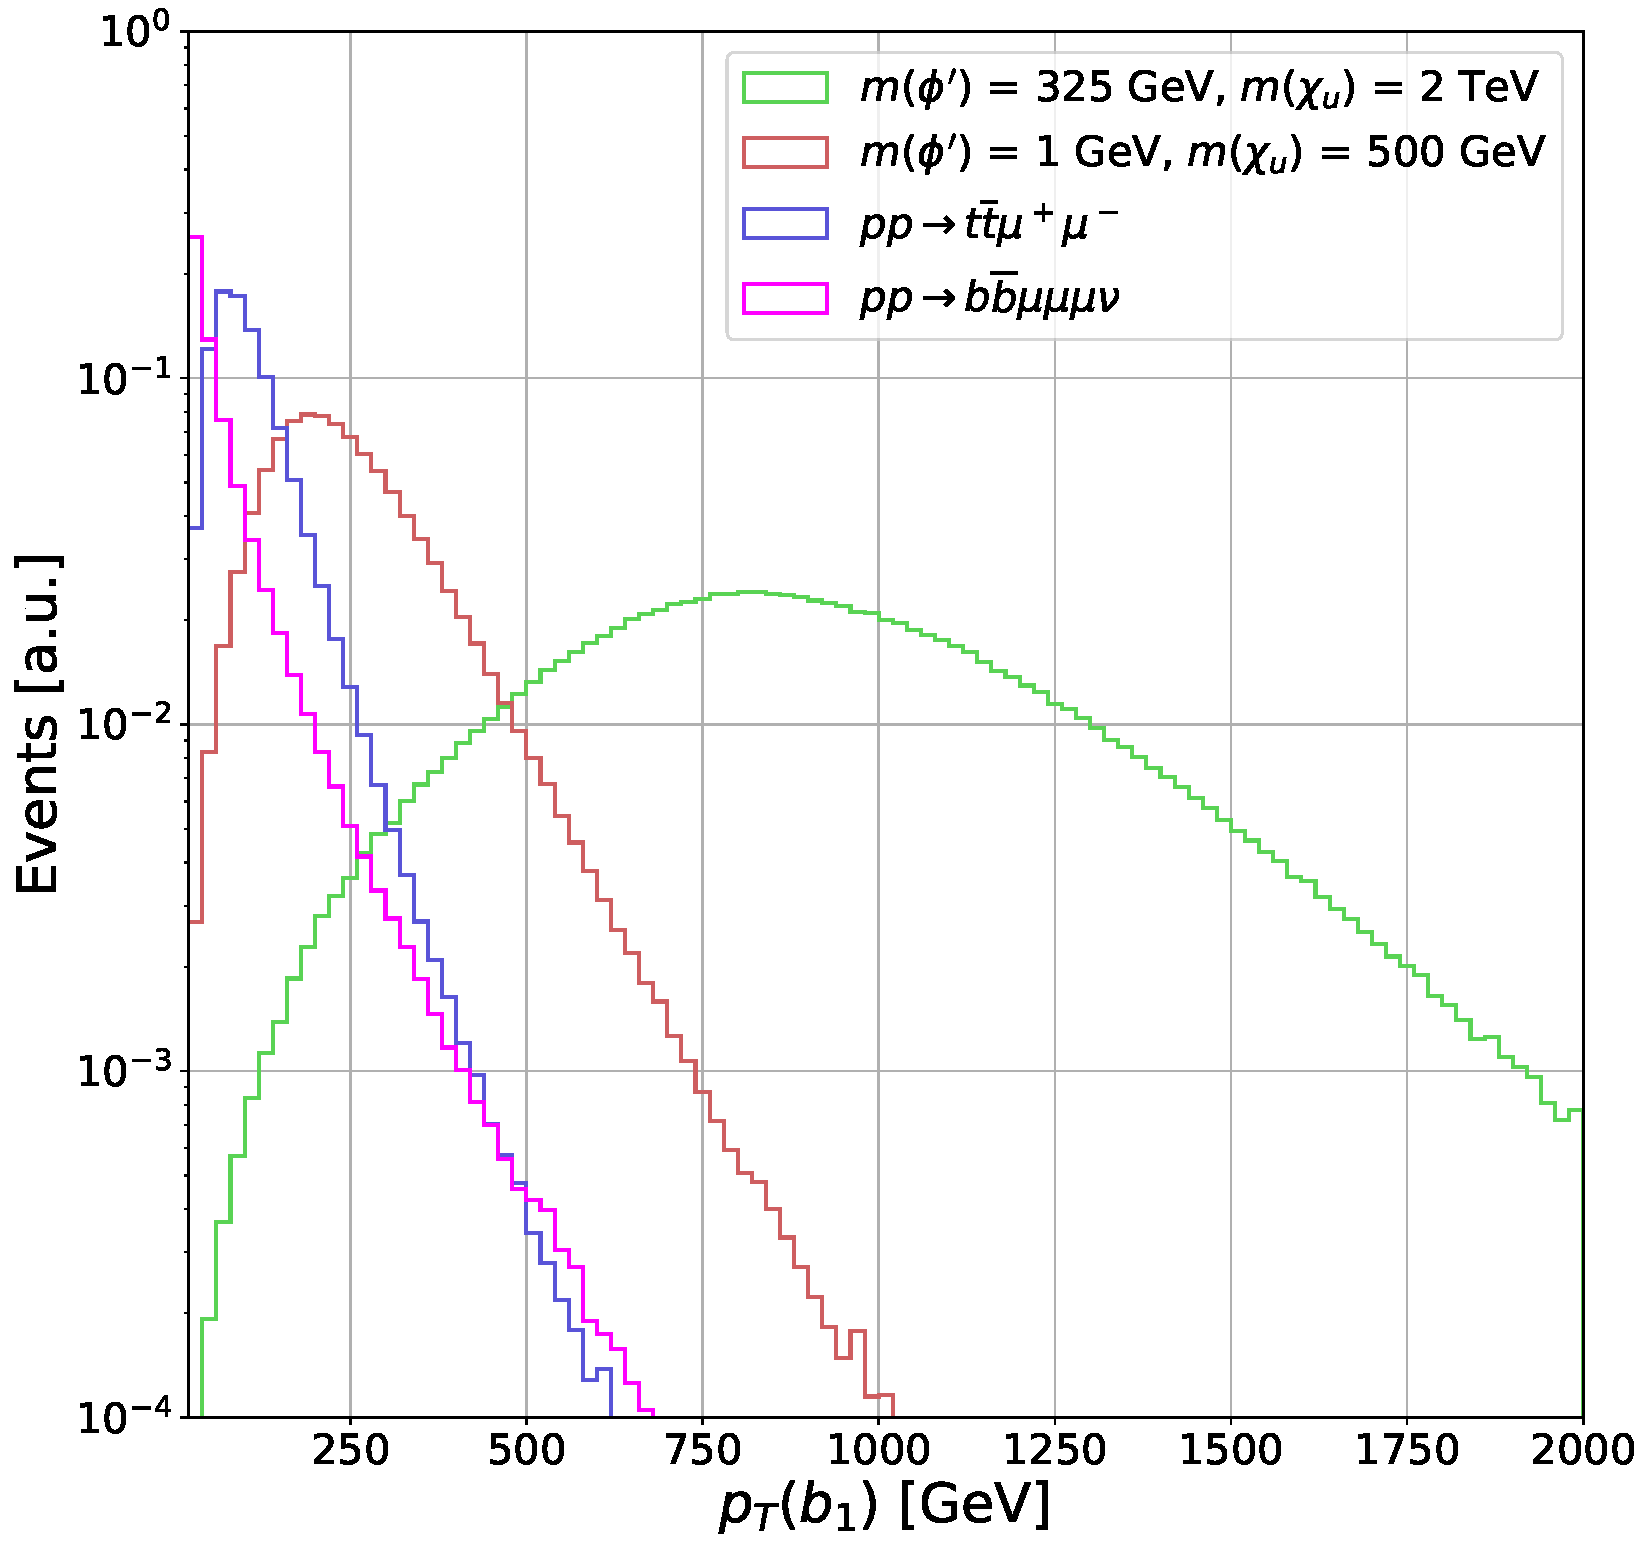
\includegraphics[width=.75\linewidth]{Images/PT_b1.pdf}
\caption{Transverse momentum distribution of the leading \textrm{b}-quark jet candidate. The distributions are shown for the two main SM background processes and two signal benchmark points.\label{fig:pTb1}}
\end{figure}

\begin{figure}
\centering
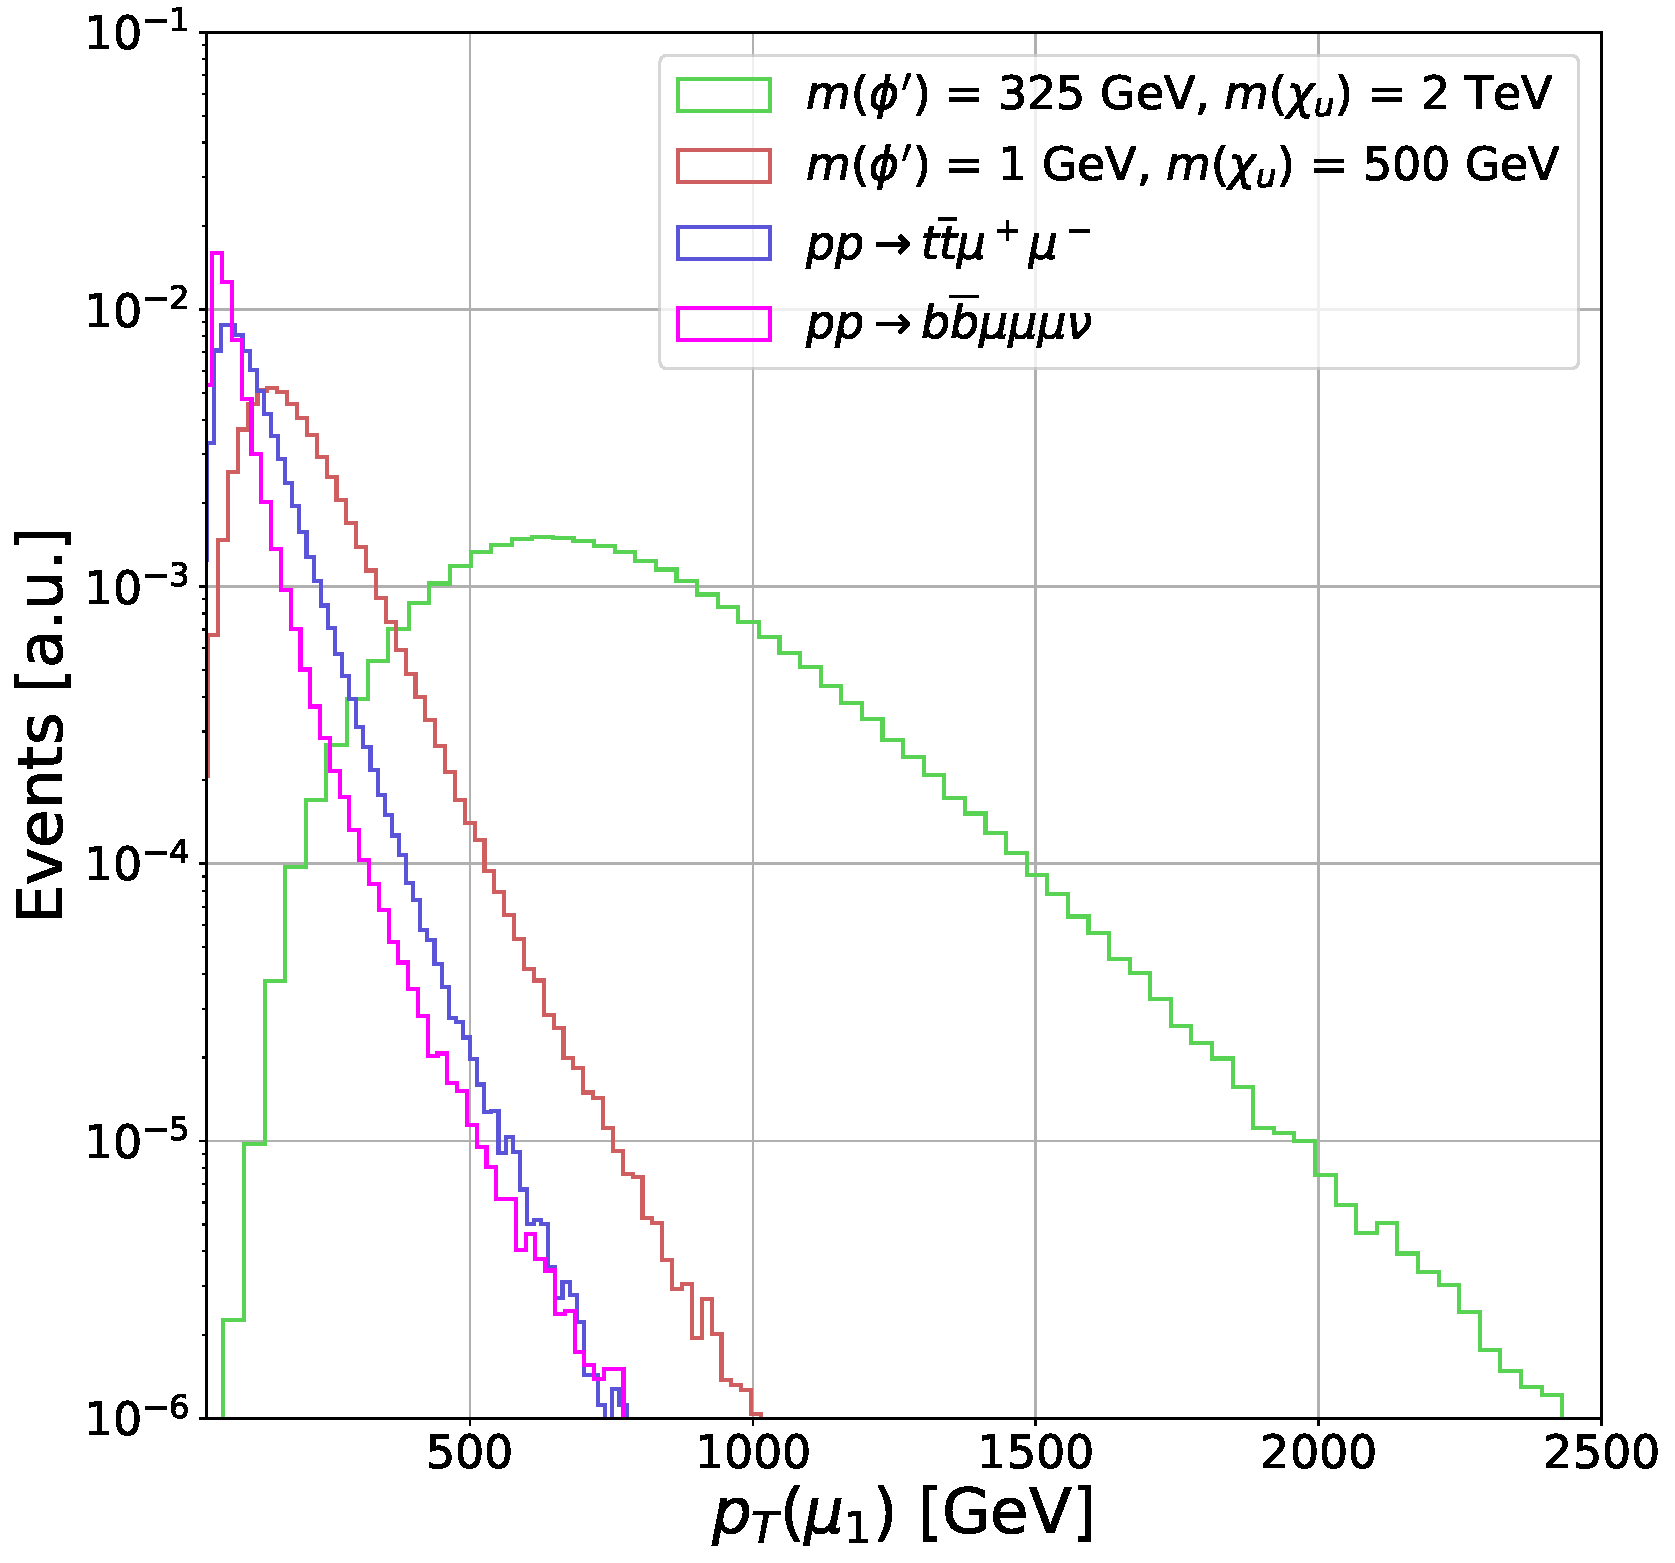
\includegraphics[width=.75\linewidth]{Images/PT_mu1_1.pdf}
\caption{Transverse momentum distribution of the leading muon candidate. The distributions are shown for the two main SM background processes and two signal benchmark points.\label{fig:pTmu1}}
\end{figure}


As can be seen from Fig.~\ref{fig:_mu12}, the $\phi'$ mass can be reconstructed through its associated muon decay pair, which is observed as a peak in the $m(\mu_{1}, \mu_{2})$ distribution around the expected $m(\phi')$ value, and has low- and high-mass tails which are a consequence of cases where the leading and/or subleading muon is not from the $\phi'$ decay, but rather from the associated $\mathrm{W}$ boson from the $\chi_{\mathrm{u}}$ decay. For the backgrounds, muons come from \textrm{Z} (\textrm{W}) decays. Therefore, the $m(\mu_{1}, \mu_{2})$ background distributions show a peak near $m_{\mathrm{W/Z}}$, combined with a broad distribution indicative of the combination of two muon candidates from different decay vertices. We note that the $\phi'\to\mu^{+}\mu^{-}$ decay width depends on the square of the $\phi'\to\mu^{+}\mu^{-}$ coupling and  $\frac{m_{\mu}^{2}}{m_{\phi'}^{2}}$ and is thus suppressed by the relatively small muon mass. For the new physics phase space considered in this paper, the $\phi'$ decay width is less than 1\% of the $\phi'$ resonant mass. Furthermore, as indicated previously, the signal/background interference effects are small and negligible compared to effects from experimental resolution. Therefore, the width of the $m(\mu_{1}, \mu_{2})$ signal distributions is driven by the experimental resolution in the reconstruction of the muon momenta, as well as the probability that the two leading muons are the correct pair from the $\phi'$ decay. Since the probability that the two highest-$p_{\mathrm{T}}$ muons are the correct pair from the $\phi'\to\mu^{+}\mu^{-}$ decay depends on $m(\phi')$ and $m(\chi_\mathrm{u})$, it is important to include all possible combinations of dimuon pairs (i.e., $m(\mu_{1}, \mu_{3})$ and $m(\mu_{2}, \mu_{3})$) in the training of the BDT. 

Fig.~\ref{fig:pTb1} shows the  distribution for the \textrm{b}-jet candidate with the highest $p_{\mathrm{T}}$, $p_{\mathrm{T}}(\mathrm{b}_1)$, for the same simulated samples shown in Fig.~\ref{fig:_mu12}. Based on the signal topology and our choice of parameter space (i.e., $m_{\chi_\mathrm{u}} > m_{\mathrm{t}}$), it is expected that the leading $\mathrm{b}$-jet candidate comes from the $\chi_\mathrm{u}$ decay, with an average $p_{\mathrm{T}}$ close to $\frac{m_{\chi_\mathrm{u}} - m_{\mathrm{W}}}{2}$, as observed in Fig.~\ref{fig:pTb1}. For the $\mathrm{t} \overline{\mathrm{t}} \mu^{+}\mu^{-}$ background, the \textrm{b}-jet candidates come from top-quark decays. Therefore, their average transverse momentum is expected to be $\frac{m_{\mathrm{t}} - m_{\mathrm{W}}}{2} \approx 45$~\textrm{GeV}, as observed in Fig.~\ref{fig:pTb1}. On the other hand, the \textrm{b}-jet candidates for the $\mathrm{b} \overline{\mathrm{b}}\mu\mu\mu\nu$ background can come from off-mass-shell $\mathrm{Z}^{*}/\gamma^{*}$, and thus typically have an even softer spectrum in comparison to the $\mathrm{t} \overline{\mathrm{t}} \mu^{+}\mu^{-}$ background.

Fig.~\ref{fig:pTmu1} shows the  distribution for the muon candidate with the highest $p_{\mathrm{T}}$, $p_{\mathrm{T}}(\mu_{1})$. Similar to Fig.~\ref{fig:pTb1}, when $m(\chi_\mathrm{u}) > m_{\mathrm{t}}$ it is expected that the leading muon candidate comes from the $\chi_\mathrm{u}$ decay, with an average $p_{\mathrm{T}}$ of approximately $\frac{m(\chi_\mathrm{u}) - m_{\mathrm{W}}}{4}$, as observed in Fig.~\ref{fig:pTmu1}. For the major SM backgrounds, the muon candidates come from Z/W/$\gamma^{*}$ decays. Therefore, their average transverse momentum is expected to be much lower, $\frac{m_{\mathrm{Z/W}}}{4} \approx 40-45$~\textrm{GeV}. This kinematic feature provides a nice handle to discriminate high $m(\chi_\mathrm{u})$ signal events amongst the large SM backgrounds, which have lower average $p_{\textrm{T}}(\mu)$ constrained by the SM weak boson masses.

In addition to these aforementioned variables in Figures~\ref{fig:_mu12}-\ref{fig:pTmu1}, several other kinematic variables were included as inputs to the BDT algorithm. In particular, 27 such variables were used in total, and these included the momenta of $\mathrm{b}$ and muon candidates; invariant masses of pairs of muons; angular differences between $\mathrm{b}$ jets and between the muons. Fig.~\ref{fig:feature_importance} shows the features that are used for training the machine learning models and their importance for a benchmark point.

\begin{figure}
\centering
  \centering
  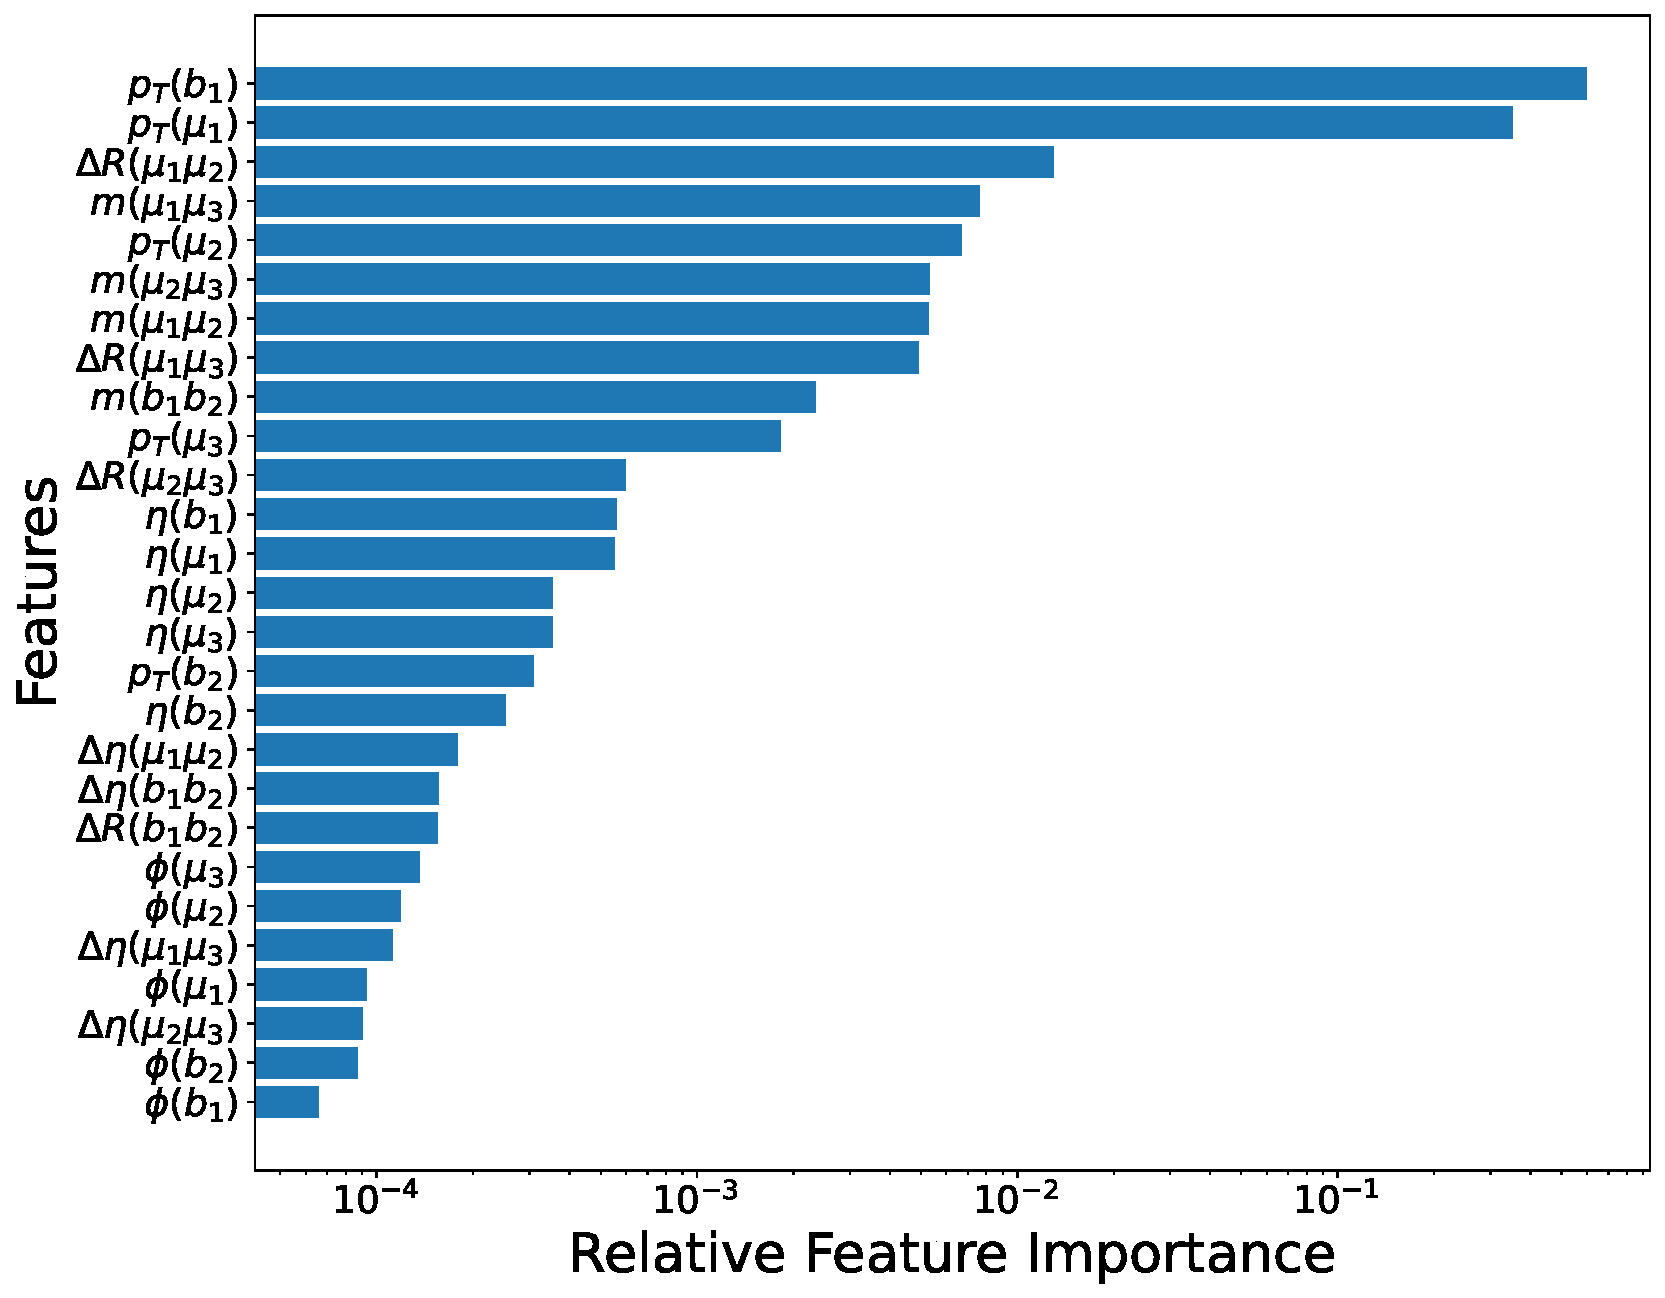
\includegraphics[width=.85\linewidth]{Images/feature_importance.pdf}
  \caption{Relative importance of features in training for a benchmark signal scenario with $m(\phi')=325\, \mathrm{GeV}$ and $m(\chi_\mathrm{u})=2000\, \mathrm{GeV}$.}
  \label{fig:feature_importance}
\end{figure}

As mentioned above, the variables $m(\mu_{i}, \mu_{j})$ for $i, j \neq 1$ provide some additional discrimination between signal and background when the leading muons are not a $\phi'$ decay candidate. The angular separation variables, such as $\Delta R(\mu_{i}, \mu_{j})$, are designed to be sensitive to lower mass $\phi'$, since the low rest mass of those particles means they acquire more boost, and thus smaller angular separation $\Delta R$ between the muon candidates. The trained BDT returns the discriminating power of each of its inputs, and the feature importance for each variable is shown in Fig.~\ref{fig:feature_importance} for a signal benchmark point with $m(\phi')=325\, \mathrm{GeV}$ and $m(\chi_\mathrm{u})=2000\, \mathrm{GeV}$.

Fig.~\ref{fig:xgboostout} shows  the distributions for the output of the BDT algorithm, normalized to unity, for the representative signal benchmark point of $m(\phi') = 1\, \mathrm{GeV}$, $m(\chi_\mathrm{u}) = 0.5\, \mathrm{TeV}$ and the two dominant backgrounds. The output of the BDT algorithm is a value between 0 and 1, which quantifies the likelihood that an event is either background-like (BDT output near $1$) or signal-like (BDT output near $0$). Fig.~\ref{fig:ROC} illustrates the true positive rate (TPR), defined as the probability of correctly selecting signal events using the BDT output, plotted against the false positive rate (FPR), defined as the probability of incorrectly selecting background events. For example, for $m(\phi') = 100\, \mathrm{GeV}$ and $m(\chi_\mathrm{u}) = 500\, \mathrm{GeV}$, when signal events are selected at $65$\% probability, the background is selected at about $10^{-3}$ probability. We note that the primary discriminating feature between the signal and background is the boosted b-jet $p_T$ coming from the $\chi_u$ vector-like quark. The $p_T$ of said b jet increases with $m(\chi_\mathrm{u})$, peaking at around $[m(\chi_\mathrm{u}) - m(\textrm{W})] / 2$. This enhanced boost increases the separation between signal and background, improving the performance of the BDT algorithm as $m(\chi_\mathrm{u})$ increases. 

\begin{figure}
\centering
  \centering  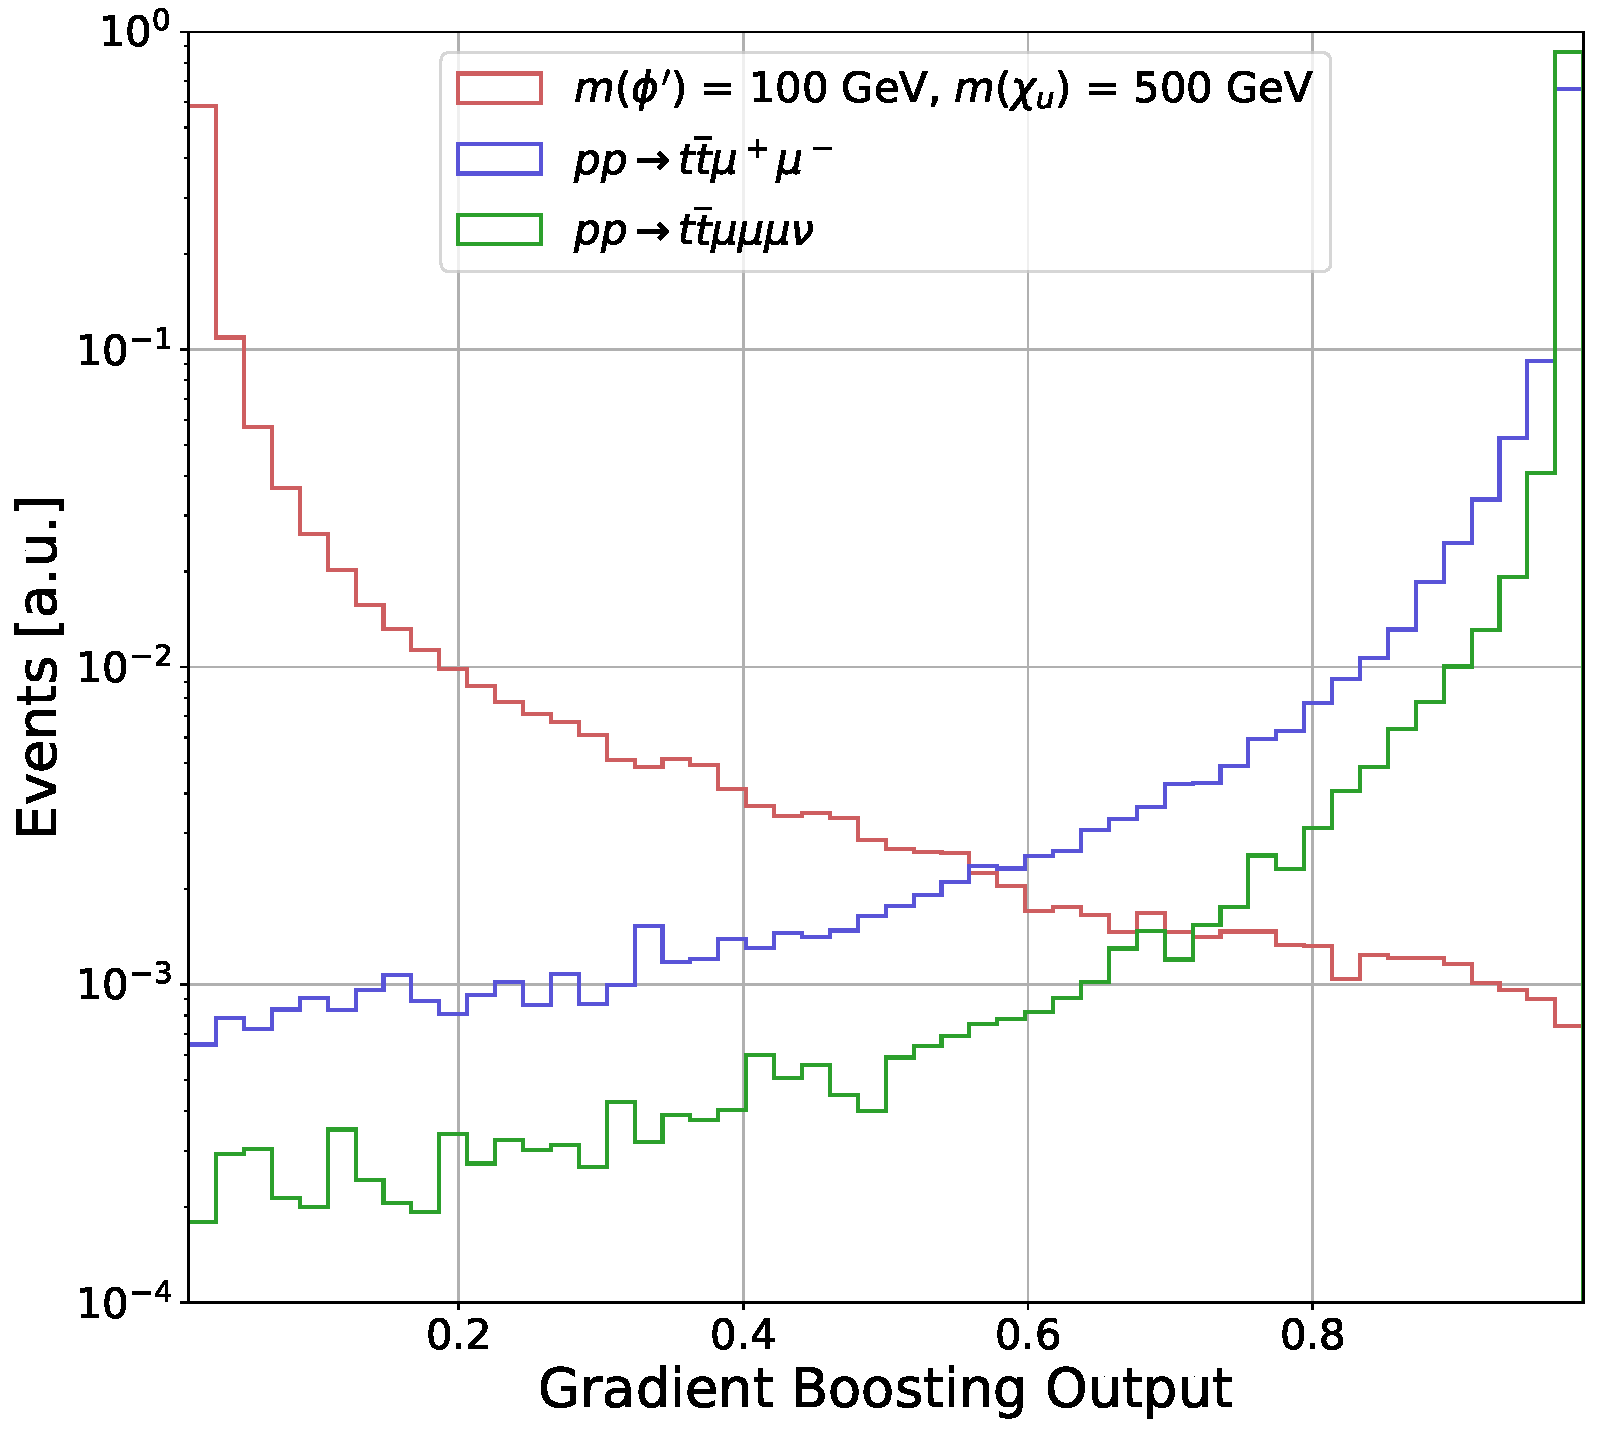
\includegraphics[width=.75\linewidth]{Images/XGB_output.pdf}
  \caption{Output of the gradient boosting algorithm for a benchmark $m(\phi') = 100$~\textrm{GeV} and $m(\chi_\mathrm{u}) = 500\, \mathrm{GeV}$ signal, and dominant backgrounds. The distributions are normalized to unity.}
  \label{fig:xgboostout}
\end{figure}


\begin{figure}
\centering
  \centering
  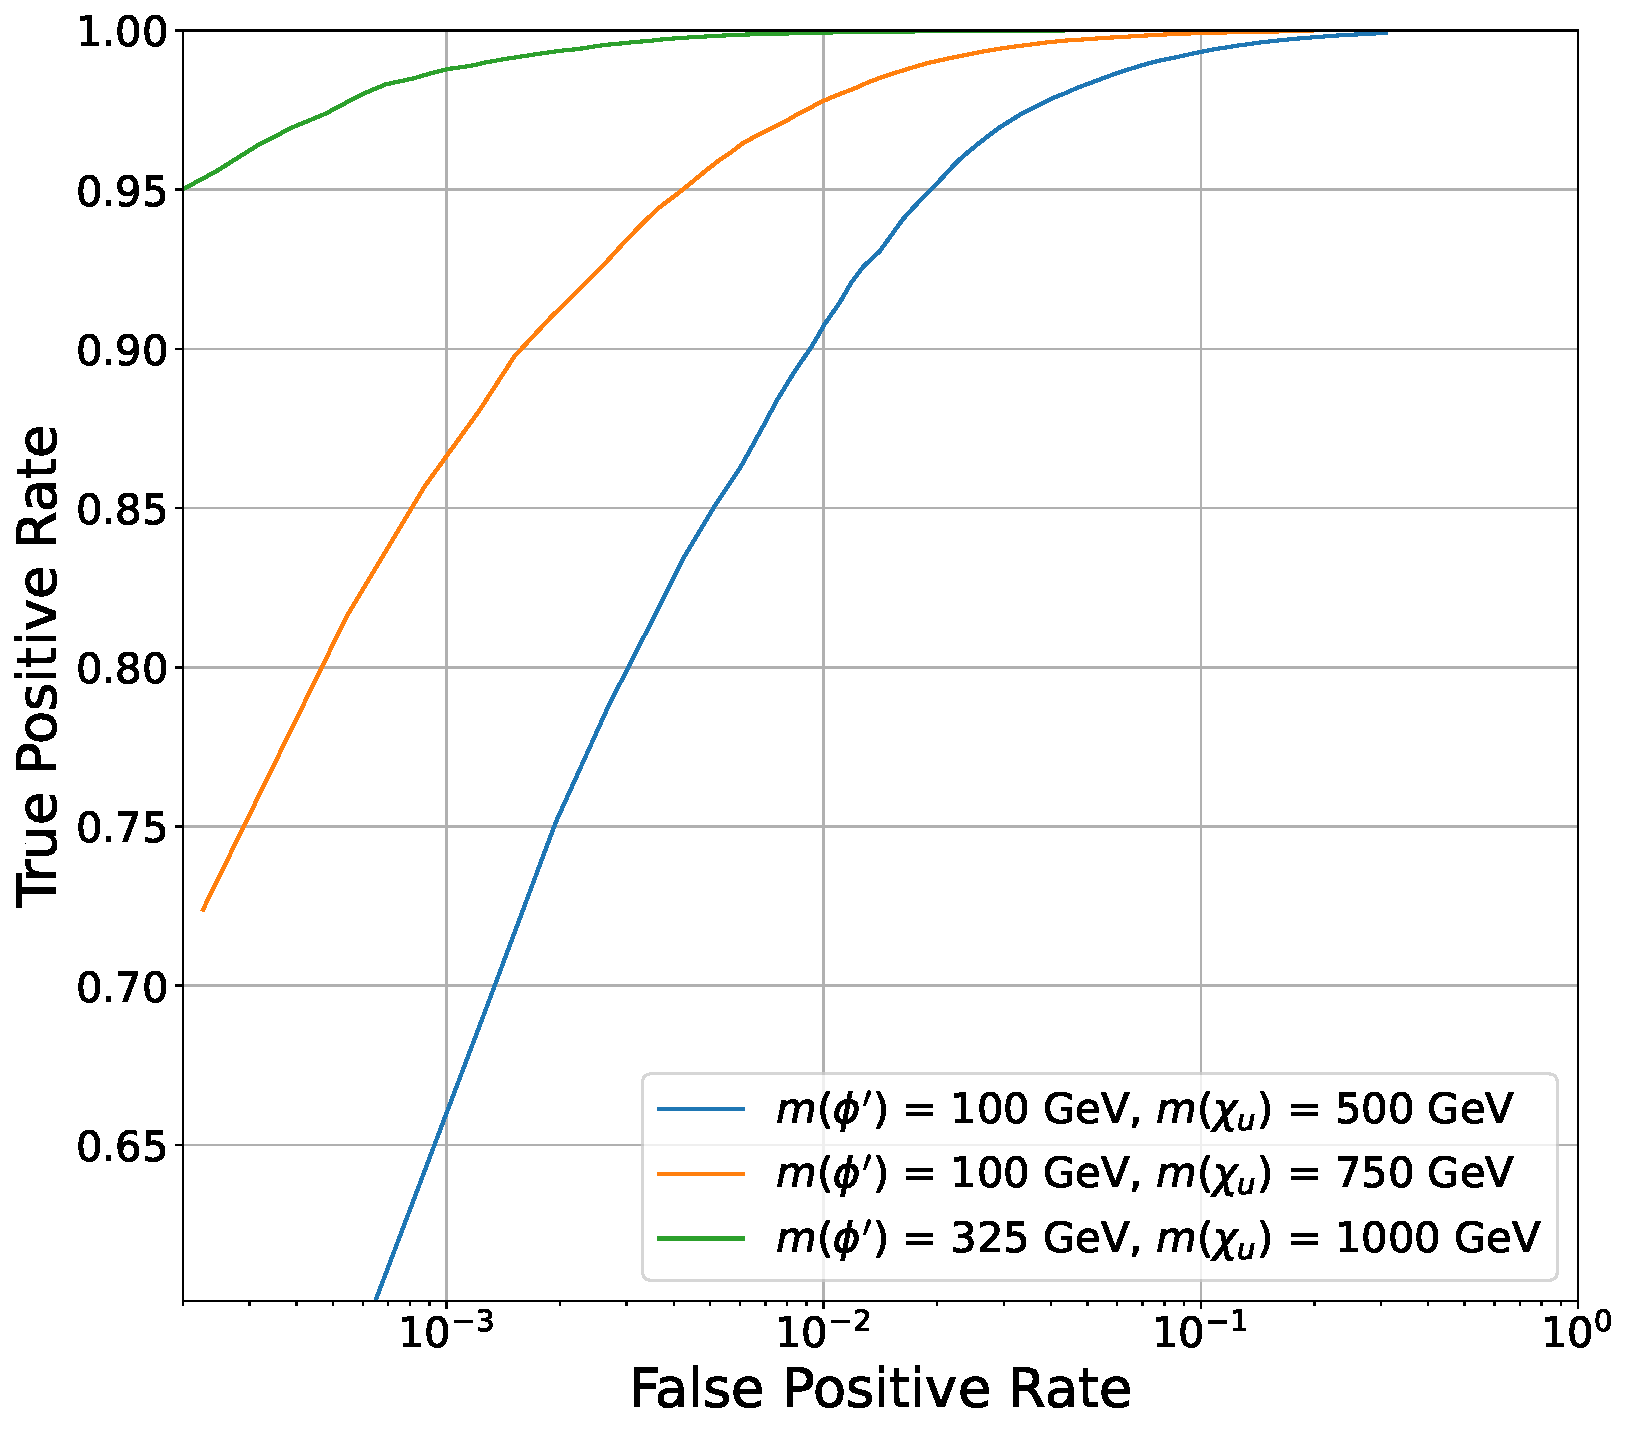
\includegraphics[width=.85\linewidth]{Images/ROC_Curve.pdf}
  \caption{Receiver operating characteristic curve of the BDT algorithm for three different signal benchmark scenarios.}
  \label{fig:ROC}
\end{figure}


The outputs from the BDT machine learning algorithm are used to perform a profile-bin likelihood analysis to estimate the signal significance for a luminosity of $3000\,\mathrm{fb^{-1}}$, corresponding to the expected amount of collected data by the end of the LHC era. For this purpose, the BDT distributions are normalized to cross section times pre-selection efficiency times luminosity for the different signal models. The significance is then calculated using the expected bin-by-bin yields of the BDT output distribution in a profile likelihood fit, using the ROOTFit~\parencite{Butterworth:2015oua} package developed by CERN. The expected signal significance $Z_\text{sig}$ is estimated using the probability of obtaining the same test statistic for the  signal plus background and the signal-null hypotheses, defined as the local $p$-value. Similar to Refs.~\parencite{Florez:2021zoo, Florez:2019tqr, Florez:2018ojp, Florez:2017xhf, VBFZprimePaper, Florez:2016lwi, Leonardi_2020}, the significance  corresponds to the point where the integral of a Gaussian distribution between $Z_\text{sig}$ and $\infty$ results in a value equal to the local $p$-value. The estimation of $Z_\text{sig}$ incorporates  systematic uncertainties. The uncertainty values have been included as nuisance parameters, considering lognormal priors for normalization and Gaussian priors for uncertainties associated with the modeling of the shapes similar to Refs.~\parencite{natalia2021longtermlhcdiscoveryreach, PhysRevD.103.095001}. 

The systematic uncertainties that have been included result from experimental and theoretical constraints.   A 1-5\% systematic uncertainty, depending on the simulated MC sample, has been included to account for the choice of Parton Distribution Function (PDF) set. The systematic uncertainty effect was incorporated following the PDF4LHC~\parencite{Butterworth:2015oua} recommendations. This systematic uncertainty has a small impact on the expected event yields for signal and background, but it does not affect the shape of the BDT output distribution. We additionally considered theoretical uncertainties related to the absence of higher-order contributions to the signal cross sections, which can change the pre-selection efficiencies and the shapes of kinematic variables used as inputs to the BDT algorithm. This uncertainty was calculated by varying the renormalization and factorization scales by $\times 2$, and studying the resulting change in the bin-by-bin yields of the BDT distributions. They are found to be at most $2$\% in a given bin. 
%Additional theoretical uncertainties were taken into account, including the potential impact of higher-order contributions to the signal cross sections. These contributions can influence the pre-selection efficiency and shapes of kinematic distributions utilized by the BDT algorithm. The uncertainty associated with this is determined by adjusting the renormalization and factorization scales by a factor of two relative to the nominal value and considering the complete change in the bin-by-bin yields of the BDT output distribution. The maximum impact of these uncertainties in a given bin is found to be 1-3\%. 

Regarding experimental uncertainties, following experimental measurements from CMS on the estimation of the integrated luminosity, a conservative $3$\% effect has been included~\parencite{lumiRef}. A $5$\% systematic uncertainty associated with the reconstruction and identification of $\mathrm{b}$-quark jets has been included, independent of $p_\mathrm{T}$ and $\eta$ of the $\mathrm{b}$-jet candidates. According to Ref.~\parencite{CMSbtag}, this uncertainty is correlated between signal and background processes with genuine  \textrm{b}-jets and is also correlated across BDT bins for each process. For muons, we include a $2$\% uncertainty associated with the reconstruction, identification, and isolation requirements, and a $3$\% systematic uncertainty to account for scale and resolution effects on the momentum and energy measurement. 
%For muon reconstruction, identification, and isolation requirements, there is a 1-2\% uncertainty, while a 1-3\% systematic uncertainty is applied to variations in energy/momentum scale and resolution. 
We consider jet energy scale uncertainties ranging from $2-5$\%, contingent on $\eta$ and $p_\mathrm{T}$, resulting in shape-based uncertainties on the BDT output distribution. Jet energy scale uncertainties were assumed to range from $1-5$\%, contingent on $\eta$ and $p_\mathrm{T}$. These assumptions lead to shape-based uncertainties on the BDT output distribution, varying from $1-2$\%. Additionally, we include  a $10$\% systematic uncertainty to account for errors in the signal and background predictions. Considering all the various sources of systematic uncertainties, our conservative  estimate yields a total effect of about $20$\%. 

\begin{figure}[]
\centering
  \centering
  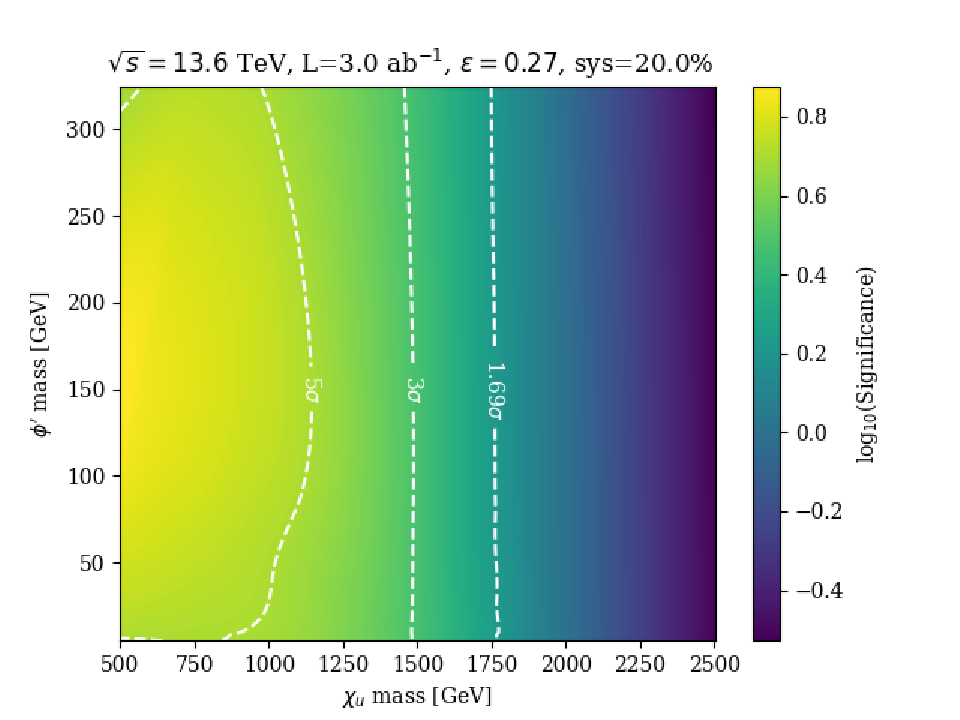
\includegraphics[width=.95\linewidth]{Images/significance.pdf}
  \caption{Signal significance for the high luminosity LHC era, considering with $3000$  $\mathrm{fb}^{-1}$ of collected data.}
  \label{fig:/significance_3000}
\end{figure}

Fig.~\ref{fig:/significance_3000} shows the expected signal significance considering an integrated luminosity of $3000$ $\mathrm{fb^{-1}}$. The significance is shown as a heat map in a two-dimensional plane for different $\phi'$ and $\chi_{\mathrm{u}}$ masses. The x-axis corresponds to $m(\chi_\mathrm{u})$, the y-axis to $m(\phi')$, and the heat map to log$_{10}(\mathrm{Z}_{sig})$. The white dashed lines are contours of constant signal significances of $1.69 \sigma$,  $3\sigma$ and  $5\sigma$ to represent regions of possible exclusion, evidence of new physics, and discovery, respectively. Under these conditions, $\phi'$ ($\chi_{\mathrm{u}}$) masses ranging from $1$ to $325$ \textrm{GeV} ($500$ to $1800$ \textrm{GeV}) can be probed. The range for a discovery with $5\sigma$ signal significance varies from $\chi_{\mathrm{u}}$ masses from $m(\chi_{\mathrm{u}}) = 770$-$1100$ \textrm{GeV}, depending  $m(\phi^{'})$. For large $m(\chi_\mathrm{u})$, the significance is almost independent of $m(\phi')$ because the primary discriminating feature—the boosted $b$-quark originating from $\phi'$—is driven predominantly by the large $m(\chi_\mathrm{u})$, with the kinematic impact of $m(\phi')$ being relatively negligible.



\section{Discussion}\label{sec:discussion}

The LHC will continue to run with pp collisions at $\sqrt{s} = 13.6$~\textrm{TeV} for the next decade. Given the increase in the integrated luminosity expected from the high-luminosity program, it is important to consider unexplored new physics phase space that diverges from the conventional assumptions made in many BSM theories, and which could have remained hidden in processes that have not yet been thoroughly examined. It is additionally crucial to explore advanced analysis techniques, in particular the use of artificial intelligence algorithms, to enhance the probability of detecting these rare corners where production cross sections are lower and discrimination from SM backgrounds is difficult. 

In this work, we examine a model based on a $U(1)_{T^3_R}$ extension of the SM, which can address various conceptual and experimental issues with the SM, including the mass hierarchy between generations of fermions, the thermal dark matter abundance, and the muon $g - 2$, $R_{(D)}$, and $R_{(D^*)}$ anomalies. This model contains a light scalar boson $\phi'$, with potential masses below the electroweak scale, and~\textrm{TeV}-scale vector-like quarks $\chi_\mathrm{u}$. We consider the scenario where the scalar $\phi'$ has family non-universal fermion couplings and $m(\phi') \ge 1$~\textrm{GeV}, as was suggested in Ref.~\cite{Dutta2020}, and thus the $\phi^{\prime}$ can primarily decay to a pair of muons. Previous works in Refs.~\cite{Dutta2023, Banerjee_2016} considered scenarios motivating a search methodology with a merged diphoton system from $\phi' \to \gamma\gamma$ decays. The authors of Ref~\cite{Dutta2023}, in which $m(\phi') < 1$~\textrm{GeV},  indeed pointed out that if the $\phi'$ is heavier than about 1~\textrm{GeV}, then decays to $\mu^+ \mu^-$ can become the preferable mode for discovery, which is the basis for the work presented in this paper. We further note that the final state topology studied in this paper would represent the most important mode for discovery at $m(\phi') < 2 m_{\mathrm{t}}$ where the $\phi' \to \mathrm{t\bar{t}}$ decay is kinematically forbidden. 

The main result of this paper is that we have shown that the LHC can probe the visible decays of new bosons with masses below the electroweak scale, down to the~\textrm{GeV}-scale, by considering the simultaneous production of heavy QCD-coupled particles, which then decay to the SM particles that contain large momentum values and can be observed in the central regions of the CMS and ATLAS detectors. The boosted system combined with innovative machine learning algorithms allows for the signal extraction above the lower-energy SM background. The LHC search strategy described here can be used to discover the prompt decay of new light particles.  An important conclusion from this paper is that the detection prospects for low-mass particles are enhanced when it is kinematically possible to simultaneously access the heavy degrees of freedom which arise in the UV completion of the low-energy model.  This specific scenario in which the couplings of the light scalars are generationally dependent, with important coupling values to the top quark, is an ideal example which would be difficult to directly probe at low energy beam experiments.

The proposed data analysis represents a competitive alternative 
to complement searches already being conducted at the LHC, allowing us to probe $\phi'$ masses from 1 to 325 \textrm{GeV}, for $m(\chi_{\mathrm{u}})$ values up to almost 2~\textrm{TeV}, at the HL-LHC. Therefore, we strongly encourage the ATLAS and CMS Collaborations to consider the proposed analysis strategy in future new physics searches. 